\documentclass{article} % For LaTeX2e


%%%
% STANDARD PREAMBLE
%%%
% https://tex.stackexchange.com/questions/68821/is-it-possible-to-create-a-latex-preamble-header
\usepackage{/Users/miw267/Repos/latex_preamble/preamble}


%%%
% PREAMBLE SPECIFIC TO THIS DOC
%%%

%%% 
% EXPONENTIAL FAMILY QUANTITIES
%%%

% General exponential family
\newcommand{\obs}{\+x}
\newcommand{\obsScalar}{x}
\newcommand{\obsCaps}{X}
\newcommand{\normalizerFunction}{Z}
\newcommand{\logNormalizerFunction}{a}
\newcommand{\sufficientStatsFunction}{\+s}
\newcommand{\carrierDensity}{h}
\newcommand{\meanParam}{\+\mu}

% Parameters
\newcommand{\param}{\+\theta}
\newcommand{\paramSpace}{\Theta}
\newcommand{\naturalParam}{\+\eta}
\newcommand{\naturalParamSpace}{H}

%Relating EM step and ordinary gradient
\newcommand{\transformationMatrixGradientToEMStep}{\+P}
\newcommand{\EMmap}{\+M}

% EF for a single observation, from which we take iid draws.
\newcommand{\logNormalizerFunctionForSingleSample}{\wt{a}}
\newcommand{\sufficientStatsFunctionForSingleSample}{\wt{\sufficientStatsFunction}}
\newcommand{\carrierDensityForSingleSample}{\wt{\carrierDensity}}


%%% 
% OTHER QUANTITIES
%%%


%%% CONTROL SIZE OF BLOCK MATRICES
% Reference: https://tex.stackexchange.com/questions/14071/how-can-i-increase-the-line-spacing-in-a-matrix

\makeatletter
\renewcommand*\env@matrix[1][\arraystretch]{%
  \edef\arraystretch{#1}%
  \hskip -\arraycolsep
  \let\@ifnextchar\new@ifnextchar
  \array{*\c@MaxMatrixCols c}}
\makeatother
 
%%% MARKOV RANDOM FIELDS 
\newcommand{\selfpotential}{\phi}
\newcommand{\edgepotential}{\psi}

%%% HIDDEN MARKOV MODEL
\newcommand{\state}{x}

%%% BAYESIAN LINEAR REGRESSION
\newcommand{\new}{\text{new}}
\newcommand{\betaML}{\wh{\+\beta}_{\text{ML}}}

%%% EMISSIONS PARAMETER
% (Used in posterior predictives section, since this was copied from the changepoint_notes repo)
\newcommand{\emissionsParam}{\param}






\begin{document}

%%%% UNTOGGLE FOR PUBLIC RELEASE
%\renewcommand{\redfootnote}[1]{}
%\renewcommand{\red}[1]{} 
%\renewcommand{\blue}[1]{} 


\title{Exponential Families} 

\maketitle
\tableofcontents
\newpage 

\section{Exponential Families} \label{sec:ef}

We are interested in  exponential families primarily because they makes inference easier.   When a problem can be cast within the exponential family framework,  inference can be tied to general principles,  and parameter updates often have nice interpretations.    This is true regardless of whether we're doing frequentist inference (such as maximum likelihood) or Bayesian inference.    Bayesian inference with exponential family likelihoods tends to be especially nice,  as all exponential family likelihoods have conjugate priors,  and distributions with conjugate priors are often also exponential families \cite{bernardo2009bayesian}. \redfootnote{TODO:  Get clearer on the relationship.  There is a brief discussion on this in \cite{bernardo2009bayesian}.  An answer from mathstackexchange at \url{https://stats.stackexchange.com/questions/176668/can-anyone-explain-conjugate-priors-in-simplest-possible-terms} gives a promising quote, although I do not know the source: ``Outside this exponential family setting, there is no non-trivial family of distributions with a fixed support that allows for conjugate priors. This is a consequence of the Darmois-Pitman-Koopman lemma." }   More complicated models may not be exponential families,  but may have exponential family complete conditional distributions;  in such situation,  we can appeal to exponential family formalisms to more easily work out inference schemes for expectation maximization,  variational inference,  or Gibbs sampling.   

\subsection{Definitions}

\begin{definition}
We can define an \textit{exponential family} as a set of probability distributions, indexed by natural parameter $\eta \in \naturalParamSpace$,%\redfootnote{TODO: Add restriction on parameter space so that the density is normalizable}  
 whose probability density functions with respect to measure $\mu$ on $\X$ have the following form
\begin{align}
 p_\eta(x) = \carrierDensity(x) \exp \{ \eta^\top \sufficientStatsFunction(x) - \logNormalizerFunction(\eta)\} 
\label{eqn:exponential_family_natural}
 \end{align}
where $\sufficientStatsFunction  : \X \to \R^p$ is the \textit{sufficient statistics function}, $\carrierDensity : \X \to \R$ is the \textit{carrier density}, $\eta \in \naturalParamSpace \subset \R^p$ is the \textit{natural parameter},  and $\logNormalizerFunction : \naturalParamSpace \to \R$ is a strictly convex and $C^{\infty}$ differentiable real-valued function known as the \textit{log normalizer} or \textit{log partition function};  that is $\logNormalizerFunction(\eta) = \log Z(\eta)$ where 
\begin{equation}
\label{eqn:partition_function}
 Z(\eta) := \ds\int  \carrierDensity(x) \exp \{ \eta^\top \sufficientStatsFunction(x)  \} \; \mu(dx)	
\end{equation}
%and so $a$ is determined by the other components of density. 
%TODO add in interpetation as \textit{cumulative generating function};


We refer to $\mu$ as the \textit{base measure}.\footnote{Some presentations use the term ``base measure" to refer to $\carrierDensity(x)$, but that is an abuse of notation, as $\carrierDensity$ is not a measure.}  Typically $\mu$ is the Lesbesgue measure or counting measure.  If $\mu$ is the Lesbesgue measure, then the density $p_\eta$ is a probability density function.  If $\mu$ is the counting measure, then the density $p_\eta$ is a probability mass function.\footnote{If measure theory is off-putting, just take $\mu$ to be the Lesbesgue measure for continuous random variables, in which case one can remove it from the equation, and simply write $Z(\eta) := \ds\int  \carrierDensity(x) \exp \{ \eta^\top \sufficientStatsFunction (x)  \} \; dx $, and take $\mu$ to be the counting measure for discrete random variables, in which case one can write $Z(\eta) := \ds\sum_{x \in \X} \carrierDensity(x) \exp \{ \eta^\top \sufficientStatsFunction(x)  \} $. Indeed, we will make precisely these assumptions throughout the document, unless otherwise noted. }  %\footnote{Some presentations assume Lebesgue measure on $\X$, and write \eqref{eqn:partition_function} more simply as $Z(\eta) := \ds\int  \carrierDensity(x) \exp \{ \eta^\top \sufficientStatsFunction(x)  \} \; dx $.  In contrast, presentations which allow for general measures $\mu$ (e.g. \cite{johnson2016composing}, or this one)  can simply absorb $\carrierDensity(x)$ into the measure $\mu$ and write \eqref{eqn:partition_function} as $Z(\eta) := \ds\int  \exp \{ \eta^\top \sufficientStatsFunction(x)  \} \; \mu (dx) $.  In the former case, the term \textit{carrier density} refers to $\carrierDensity(x)$ -- although this is an abuse of notation.  We use the term \textit{base measure} refers to $\mu$. Some presentations use the term ``base measure" to refer to $\carrierDensity(x)$, but that is an abuse of notation, as $\carrierDensity$ is not a measure.}  
%\redfootnote{TODO: Align more closely with Jordan, who uses integration against probability measure here.  He remarks on this somewhere in his exponential family lecture notes.   What also may be helpful is this beautiful excerpt from pp.38 of \cite{wainwright2008graphical}: `` $[...]$ we represent the probability distribution as a density $p$ absolutely continuous with respect to some measure $\eta$.   This base measure $\eta$ might be the counting measure on $\set{0, 1, ..., r-1}$,  in which case $p$ is a probability mass function; alternatively, for a continuous random vector, the base measure $\eta$ could be the ordinary Lebesgue measure on $\R$."}  
\label{def:exponential_family}
\end{definition} 


\begin{remark}\remarktitle{Alternate constructions for the exponential family.}
Observe \cite{chua2019stats} that without loss of generality, the following properties hold. 
%
\begin{alphabate} 
\item \label{item:ignorabiity_of_carrier_density} \textit{(Ignorability of the carrier density.)} We can always set $\carrierDensity(\obs) \equiv 1$ if we change $\mu$ to $\wt{\mu}$, chosen so that its Radon-Nikodym derivative with respect to $\mu$ is $\carrierDensity$. That is, we can always absorb $\carrierDensity$ into $\mu$ and write \eqref{eqn:exponential_family_natural} as  $p_\naturalParam(\obs) = \exp \{ \naturalParam^\top \sufficientStatsFunction(\obs) - \logNormalizerFunction(\naturalParam)\}$, in which case \eqref{eqn:partition_function} becomes $\normalizerFunction(\naturalParam) := \ds\int  \exp \{ \naturalParam^\top \sufficientStatsFunction(\obs)  \} \; \wt{\mu} (d\obs) $ where $\wt{\mu}(A) := \ds\int_A \carrierDensity d\mu$ for any measurable set $A$.   This observation streamlines most computations with integrals, e.g. see the proof of Prop.~\ref{prop:basic_convexity_properties_of_the_exponential_family}. 
\item \label{item:nonuniqueness_of_natural_parameter} \textit{(Non-uniqueness of natural parameter.)} Assume $M \in \R^{p \times p}$ is invertible, and define $\wt{\sufficientStatsFunction} = M \sufficientStatsFunction(\obs)$. Then defining $\wt{\naturalParam} = M^{-1} \naturalParam$ results in an equivalent family.  As a special case, $\naturalParam$ could be multiplied by a non-zero constant $c$ if $\sufficientStatsFunction(\obs)$ is divided by $c$.  Thus, a natural parameterization is not unique; we should speak of \textit{a} natural parameter,  rather than \textit{the} natural parameter.
\item \textit{(The carrier density may absorb the probability density at the zero parameter.)} We may change $\carrierDensity$ to $\wt{\carrierDensity}(\obs) = p_\+0(\obs)$, assuming that $\+0 \in \naturalParamSpace$.  Then, changing $\logNormalizerFunction(\naturalParam)$ to $\wt{\logNormalizerFunction}(\naturalParam) = \logNormalizerFunction(\naturalParam) - \logNormalizerFunction(\+0)$ results in an equivalent family.\redfootnote{TODO: Give an example of why this is useful.}
\end{alphabate}
\label{rk:alternate_constructions_for_the_exponential_family}
\end{remark}


\begin{definition}
The \textbf{natural parameter space} is the set of parameters $\naturalParam$ for which the integral \eqref{eqn:partition_function} is finite; i.e., it is $\naturalParamSpace:=\set{\naturalParam : \normalizerFunction(\naturalParam) < \infty}$.
\end{definition}

\begin{definition}
An exponential family is said to be \textbf{regular} if the natural parameter space is an open set.
\end{definition}

\begin{remark}\remarktitle{Exponential families with general (non-natural) parametrizations \cite[pp.~49]{bickel2001mathematical}, \cite{jordan2010exponential}.}
One can \textit{reparameterize} a regular exponential family with some other coordinates $\param$.  If one writes the natural parameter as a continuous function $\naturalParam(\param)$, then the density \eqref{eqn:exponential_family_natural} becomes
\begin{align}
 p_\param(\obs) = \carrierDensity(\obs) \exp \{ \naturalParam(\param)^\top \sufficientStatsFunction(\obs) - \logNormalizerFunction(\naturalParam(\param))\} 
\label{eqn:exponential_family}
 \end{align}
 The reparameterized family is regular as well, since $\param := \naturalParam^{-1}(\naturalParamSpace)$ is open.\redfootnote{TODO: Why do we define $\naturalParam$ as a function of $\param$, rather than the other way around?}
\end{remark}

\begin{remark}
Exponential family members can have intractable normalization constants.  Consider, for example,  the Ising model.  See pp. 3 of \cite{taylor2013multiparameter}.
\end{remark}


\begin{definition}
An exponential family is said to be \textbf{minimal} if the components of the sufficient statistics $\sufficientStatsFunction(\obs)$ are linearly independent ($\mu$-a.e.).\redfootnote{CHECK: This statement, when given by David Blei, made no mention of almost everywhere.  The next statement, however, which came from \cite{johnson2016composing}, does.  I attempted to align them by adding ``almost everywhere" to the linear independence claim.  Hopefully this is valid.}  That is, there must be no $\naturalParam(\param) \in \R^n \textbackslash \set{\+0}$ such that $\naturalParam(\param)^\top \sufficientStatsFunction(\obs) = 0$ ($\mu$-a.e.).\redfootnote{Is it strictly speaking necessary to assume that the parameters are real-valued? If so, why?}
\label{def:minimal_exponential_families}
\end{definition}

  An example of a non-minimal exponential family is the categorical distribution (Example \ref{ex:categorical_as_ef}).\redfootnote{Justify that the categorical distribution is non-minimal, and state how to rectify. Also demonstrate the importance of this.}\redfootnote{TODO: I believe a non-minimal EF can always be reparametrized into a minimal EF. This makes sense based on the definition, based on the categorical distribution, and based on an implication from \citet[Sec.~8.4]{jordan2010exponential}.  Justify this.}

\subsection{Examples}

Here we give examples of exponential families, showing how to derive the exponential family forms.   Note that the result of such computations are readily available for a wide variety of exponential family members (see e.g. \cite{nielsen2009statistical} or the Wikipedia page on exponential families). 

 
\subsubsection{Categorical distribution}

\begin{example}{(Categorical Distribution)}
\label{ex:categorical_as_ef} We can write the density of the categorical distribution in exponential family form. 	 Given one-hot encoded observations $\obs \in \set{0,1}^K$ and simplex-valued parameter $\pi \in \Delta_{K-1}$, we can write
\[p(\obs \cond \pi) = \prod_{k=1}^K \pi_k^{\obsScalar_k} = \exp \{ \sum_{k=1}^K \obsScalar_k \log \pi_k\} \]
 with natural parameter, $\naturalParam(\pi) = \log \pi$, the sufficient statistics $\sufficientStatsFunction(\obs) = \obs$, carrier density $\carrierDensity(\obs)=1$ and log normalizer $0$.
\end{example}

\subsubsection{Dirichlet distribution}
\begin{example}{(Dirichlet Distribution)} 
\label{ex:dirichlet_as_ef} We can write the density of the Dirichlet distribution in exponential family form:
\begin{align*}
p (\pi \cond\alpha) &= \df{\Gamma(\sum_k \alpha_k)}{\prod_k \Gamma (\alpha_k) } \pi_1^{\alpha_1 -1} \cdot \cdot \cdot \pi_K^{\alpha_K -1} \\
&= \exp \bigg\{ \sum_{k=1}^K (\alpha_k -1) \log \pi_k - \bigg[ \sum_k \log \Gamma (\alpha_k)-  \log \Gamma (\sum \alpha_k) \bigg]  \bigg\}
\end{align*}
with natural parameter $\naturalParam(\alpha) = [\alpha_1 -1, ..., \alpha_K -1]^\top$, sufficient statistics $\sufficientStatsFunction(\pi) = \log \pi = [\log \pi_1, ..., \log \pi_K]^\top$, carrier density $\carrierDensity(\pi)=1$, and log normalizer $\logNormalizerFunction(\alpha) =  \sum_k \log \Gamma (\alpha_k ) - \log \Gamma (\sum_k \alpha_k)$. 
  
\end{example} 

For an example of how the natural parametrization can help provide insight into message passing,  see Section \ref{sec:mvn_in_message_passing}.

\begin{remark} The exponential family representation of the Dirichlet, as given in Example \ref{ex:dirichlet_as_ef}, is useful when we want to compute the expectation of a log probability from a Dirichlet distributed probability vector (as happens in the derivation of LDA with variational inference; see my notes on variational inference).  

In those notes,  we see
\begin{align} 
\E [ \log \pi_k] &= \E [\sufficientStatsFunction_k(p)] \stackrel{1}{=} \df{\partial}{\partial \naturalParam_k} a(\naturalParam) \nonumber \\
&=\Psi(\alpha_k) -  \Psi(\sum_k  \alpha_k) \label{eqn:expectation_of_log_probability} 
\end{align}
where (1) uses a well-known exponential family property (see Proposition \ref{prop:expected_sufficient_statistic_as_derivative_of_log_normalizer}) and where $\Psi(\cdot)$ is the first derivative of the $\log \Gamma$ function.   It is known as the \textit{digamma function}.  $ $

% See e.g., https://zhiyzuo.github.io/Exponential-Family-Distributions/
\end{remark}

\subsubsection{Truncated normal distribution}

\begin{example}{(Truncated normal distribution)} 
\label{ex:truncated_normal_as_ef} The univariate truncated normal distribution $\TruncatedNormal(\mu,  \sigma^2,  \Omega)$ results when a normal distribution $\N(\mu,  \sigma^2)$ is truncated to some set $\Omega \in \R$. \footnote{For more information on the truncated normal,  see e.g.  \cite{burkardt2014truncated} or \url{http://parker.ad.siu.edu/Olive/ch4.pdf}.}   Note that the parameters $\mu, \sigma^2$ denote the mean and variance of the \textit{parent} normal distribution;  i.e.  if $X \sim \TruncatedNormal(\mu,  \sigma^2,  \Omega)$ then $\E[X] \neq \mu$ (unless $\Omega = \R$). 

If we assume that the truncation set is an interval $\Omega = (a,b)$ for $a,b \in \R$,  then the distribution $\TruncatedNormal(\mu,  \sigma^2,  (a,b))$ has p.d.f.

\begin{align*}
f(x ; \mu,  \sigma^2,  a,  b) = \df{\phi_{\mu, \sigma^2} (x) }{\Phi_{\mu, \sigma^2} (b)  - \Phi_{\mu, \sigma^2} (a) } \indicate{a \leq x \leq b} \labelit \label{eqn:pdf_of_normal_truncated_to_an_interval}
\end{align*} 

where $\phi_{\mu,  \sigma^2}$ and $\Phi_{\mu,  \sigma^2}$ denote the pdf and cdf,  respectively,  of a univariate normal distribution with mean $\mu$ and variance $\sigma^2$.   

If we write
\begin{align*}
f(x ; \mu,  \sigma^2,  a,  b) & = K \df{1}{\sqrt{2 \pi \sigma^2}} \exp \bp{-\half \df{(x-\mu)^2}{\sigma^2}}  \indicate{a \leq x \leq b} \\
& = K \df{1}{\sqrt{2 \pi}} \exp \bp{ - \frac{1}{2 \sigma^2} x^2 + \frac{\mu}{\sigma^2} x  + \frac{\mu^2}{\sigma^2}  - \log \sigma}  \indicate{a \leq x \leq b} 
\end{align*} 
where $K := \big( \Phi_{\mu, \sigma^2} (b)  - \Phi_{\mu, \sigma^2} (a) \big)^{-1}$,  then we see that see that  $\TruncatedNormal(\mu,  \sigma^2,  (a,b))$ belongs to the exponential family \eqref{eqn:exponential_family} where,  in this case,  we have natural parameter $\naturalParam = (\frac{1}{\sigma^2},  \frac{\mu}{\sigma^2})\top$,  sufficient statistics function $\sufficientStatsFunction(x) = (-\half x^2,  x)^\top$,  carrier density $\carrierDensity(x) =  \frac{1}{\sqrt{2 \pi}}  \indicate{a \leq x \leq b}$,  and log normalizer $a(\param) = \log K + \frac{\mu^2}{\sigma^2} - \log \sigma$.
 
\end{example}

\begin{remark}
The truncated normal distribution differs from the normal distribution only in its carrier density $\carrierDensity(x)$ and therefore log normalizer $\logNormalizerFunction(\param)$.  The natural parameter $\naturalParam$ and sufficient statistics function $\sufficientStatsFunction(x)$ are identical.   Thus,  knowing $\naturalParam$ and $\sufficientStatsFunction(x)$ is not sufficient to determine the form of the probability distribution.
\label{rk:truncated_normal_differs_from_normal_only_in_terms_of_carrier_density}
\end{remark}


\subsubsection{Inverse Gamma distribution}

\begin{example}{(Inverse Gamma Distribution)} 
\label{ex:inverse_gamma_as_ef} The Inverse Gamma distribution is the distribution of the reciprocal of a Gamma random variable.\footnote{The density of the inverse gamma can easily be obtained from the gamma density by defining the transformation $Y = \frac{1}{X} := g(X)$ and then applying the change of variables formula,  $f_Y(y) = f_X (g^{-1}(y)) | \df{d}{dy} g^{-1}(y)|$.}  We can write the density of the Inverse Gamma $\InverseGamma(\alpha,  \beta)$ distribution in exponential family form:
\begin{align*}
p (x \cond \alpha,  \beta) &= \df{\beta^\alpha}{ \Gamma (\alpha) } x^{-\alpha -1} \exp \bigg(- \df{\beta}{x} \bigg) \\
&= \exp \bigg\{ (-\alpha - 1) \log x + (- \beta) \frac{1}{x} + \log \df{\beta^\alpha}{\Gamma(\alpha)} \bigg\}
\end{align*}
with natural parameter $\naturalParam(\alpha) = [-\alpha-1,  -\beta]\top$, sufficient statistics $\sufficientStatsFunction(x) = [\log x ,  \frac{1}{x}]^\top$, carrier density $\carrierDensity(x)=1$, and log normalizer $a(\alpha,  \beta) =  \log \frac{\beta^\alpha}{\Gamma(\alpha)} $. 
  
\end{example} 

\subsubsection{Multivariate normal}

\begin{example}{(Multivariate normal)} 
\label{ex:mvn_as_ef}
We can write the density of a multivariate normal $\N(\+\mu, \+\Sigma)$ distribution in exponential form
\begin{align*}
	p(\+x \cond \+\mu, \+\Sigma) &= (2\pi)^{-d/2} |\+\Sigma |^{-1/2} \exp \bigg\{ -\half (\+x - \+\mu)^\top \+\Sigma^{-1} (\+x - \+\mu) \bigg\}  \\
& \stackrel{1}{=} (2\pi)^{-d/2} \exp \bigg\{ -\half \explaintermbrace{$-\half \vectorize (\+\Sigma^{-1})^\top \vectorize (\+x\+x^\top) $}{\+x^\top \+\Sigma^{-1} \+x} + \+x^\top \+\Sigma^{-1} \+\mu -\half \+\mu^\top \+\Sigma^{-1} \+\mu + \half \log |\+\Sigma^{-1} | \bigg\} \\
	\labelit \label{eqn:mvn_as_ef}
\end{align*} 
with natural parameter $\naturalParam(\+\mu, \+\Sigma) = \big(-\half \vectorize (\+\Sigma^{-1}) , \,  \+\Sigma^{-1} \+\mu \big) $, sufficient statistics $\sufficientStatsFunction(\+x) = \big(\vectorize (\+x \+x^\top), \+x \big)$, carrier density $\carrierDensity(\obs) = (2\pi)^{-d/2}$ and log normalizing $\logNormalizerFunction(\+\mu, \+\Sigma) =  -\half \+\mu \+\Sigma^{-1} \+\mu + \half \log |\+\Sigma^{-1} | $. 
\end{example}

\begin{remark}
From Example \ref{ex:mvn_as_ef}, we see that the natural parameters of the MVN are the \textit{precision} $\+\Sigma^{-1}$ and \textit{precision-weighted mean} $\+\Sigma^{-1} \+\mu$. 
\end{remark}

\begin{remark}
 The underbrace representation in Equation (1) is given by $\+x^\top \+\Sigma^{-1} \+x = \tr (\+x^\top \+\Sigma^{-1} \+x) = \tr (\+\Sigma^{-1} \+x \+x^\top) =\vectorize (\+\Sigma^{-1})^\top \vectorize (\+x\+x^\top)$.\footnote{Recall $\tr(\+A\+B) = \vectorize (\+A)^\top \vectorize (\+B)$.}  
\end{remark}

\begin{remark}
In Section \ref{sec:normal_data_with_non_conjugate_prior}, we use the exponential family representation to derive the updates to the mean for a Bayesian normal model with conditionally conjugate prior.
\end{remark}

\begin{remark}
\label{rk:mvn_from_ef}
Equation \eqref{eqn:mvn_as_ef} also says that if a random vector $\+x$ has a density on $\R^d$ that is proportional to $\exp \{ -\half \+x^\top \+A \+x + \+x^\top \+b\}$ for some matrix $\+A$ and vector $\+b$, then $\+x$ must be multivariate normal with covariance $\+A^{-1}$ and mean $\+A^{-1}\+b$. 
\end{remark}
	

\subsubsection{Inverse Wishart distribution}

\begin{example}{(Inverse Wishart distribution)} 
\label{ex:inverse_wishart_as_ef} The Inverse Wishart distribution (Section \ref{sec:inverse_wishart_distribution}) is the distribution of the inverse of a Wishart random variable.   We can write the density of the Inverse Wishart $\InverseWishart(\+\Psi,  \nu)$ distribution in exponential family form:
\begin{align*}
p (\+X  \cond \+\Psi,  \nu) & \stackrel{1}{=} C(\+\Psi,  \nu) \; | \+X | ^{-(\nu + p + 1)/2} \exp \bigg\{ -\half \tr (\+\Psi \+X^{-1} ) \bigg\} \\
& = \exp \bigg\{ \frac{-(\nu + p + 1)}{2}  \log | \+ X | \;  -\half \tr (\+\Psi \+X^{-1} )  \; + \log  C(\+\Psi,  \nu)   \bigg\} \\
& \stackrel{2}{=} \exp \bigg\{ \frac{-(\nu + p + 1)}{2}  \log | \+ X | \;  -\half  \ds\sum_{i,j=1}^p \+\Psi_{ij} \+X^{-1}_{ij} \; + \log  C(\+\Psi,  \nu)   \bigg\} 
\end{align*}
Equation (1) gives the standard representation of the $\InverseWishart(\+\Psi,  \nu)$ density,  where   $C(\+\Psi,  \nu)$ is the normalizing constant,  $| \cdot |$ refers to the determinant,  $\+X,  \+\Psi \in \R^{p \times p}$ are positive definite matrices,  and $\nu > p-1$.    Equation (2) uses the fact that the trace of a matrix product behaves like a dot product \eqref{eqn:trace_of_matrix_product}.      


As we see from the last line,  in the exponential family representation,  we have natural parameter $\naturalParam = [\frac{-(\nu + p + 1)}{2},  \; -\half \vectorize (\+\Psi)]^\top$, sufficient statistics $\sufficientStatsFunction(\+X) = [\log | \+X | , \vectorize (\+X^{-1})]^\top$, carrier density $\carrierDensity(\+X)=1$, and log normalizer $ \log  C(\+\Psi,  \nu)$.   
  
\end{example} 

%{eqn:trace_of_matrix_product}

\subsubsection{Gaussian Mixture Models}


For a detailed explanation of how to represent Gaussian mixture models in the exponential family, see \url{https://www.youtube.com/playlist?list=PLD0F06AA0D2E8FFBA}, videos 16.6-16.8. More generally, it can be shown that mixtures of any exponential family distributions are still in the exponential family. 


\subsubsection{Hidden Markov Models} 

\begin{example}{(Hidden Markov Models)} 
A  hidden Markov model (HMM) is a tool for representing probability distributions over sequences of observations.  The HMM assumes that the observation at time $t$ was generated by some process whose state $\state_t$ is hidden from the observer.  Moreover, it assumes that the sequence of states satisfies the \textit{Markov property}:  conditional on the current state $\state_t$, its future and past hidden states are independent.  Finally, there is a Markov property on outputs:  conditional on the current state $\state_t$, the output $y_t$ is independent of all other hidden states and outputs.\redfootnote{I might have lifted this paragraph overviewing HMM's from somewhere; check into that.}

% Note: No need to introduce the Bayesian hidden markov model here; we're just showing that the complete data likelihood is in the
% exponential family.
%
%The full generative model over the parameters, hidden state sequence $\state_{1:T}$ and observation sequence $y_{1:T}$ is
%
%\begin{align*}
%\pi &\sim \text{Dir}(\alpha^\pi) & A_k &\iid \text{Dir}(\alpha^{A_k})  & \phi_k &\iid p(\phi_k \cond \beta) \\
%\state_1 &\sim \pi & \state_{t+1} &\sim A_{\state_t} & y_t &\sim p(y_t \cond \phi_{z_t})
%\end{align*}
 
The the \textit{complete data likelihood} for the HMM is given by

\begin{align}
 p(\state_{1:T}, y_{1:T} \cond \param) &=  p(\state_1 \cond \param)  p(y_1 \cond \state_1, \param) \ds\prod_{t=2}^T p(\state_t \cond \state_{t-1}, \param) p(y_t \cond \state_t, \param) \nonumber \\
 &=  p(\state_1 \cond \pi) p(y_1 \cond \state_1, \phi) \ds\prod_{t=2}^T p(\state_t \cond \state_{t-1}, A) p(y_t \cond \state_t, \phi)   \nonumber \\
 &= \pi_{\state_1}  \; \ds\prod_{t=2}^T A_{\state_{t-1}, \state_t} \ds\prod_{t=1}^T p(y_1 \cond \phi_{\state_t}) \label{eqn:hmm_cdl_compact}
 \end{align}
 
where we have defined 

\begin{itemize}
\item $y_{1:T}=(y_1, ..., y_T)$ observed sequence
\item $\state_{1:T} =(\state_1, ...., \state_T)$: hidden state sequence ($\state_t \in \{1,...,K \}$) 
\item $\pi = \{ \pi_k \}, \pi_k = P(\state_1 = k)$: initial state distribution
\item $A=\{A_{kk'}\}, A_{kk'} = P(\state_t= k' \cond \state_{t-1}=k):$ state transition probability matrix 
\item $\phi = (\phi_k)_{k=1}^K$ a set of parameters, each governing an output distribution (also called emissions distribution) associated to each hidden state; that is, $ P(y_t \cond \state_t=k) = P(y_t \cond \phi_k)$. 
\item $\param = (\pi, A, \phi)$: model parameters
\end{itemize}


We can write the complete data likelihood \eqref{eqn:hmm_cdl_compact} as
\begin{align}
p(\state_{1:T}, y_{1:T} \cond \param) &=  \exp\bigg \{ \log p(\state_1 \cond \pi) + \ds\sum_{t=2}^T \log p(\state_t \cond \state_{t-1}, A) +  \ds\sum_{t=1}^T \log p(y_t \cond \state_t, \phi) \bigg\}  \nonumber \\
&= \exp \bigg \{ \log \pi_{\state_1}  + \ds\sum_{t=2}^T \log A_{\state_{t-1}, \state_t} + \ds\sum_{t=1}^T \log p(y_1 \cond \phi_{\state_t}) \bigg\} \nonumber \\
&=  \exp\bigg \{  \ds\sum_{k=1}^K \state_1^k \log \pi_k + \ds\sum_{t=2}^T \ds\sum_{k, k'=1}^K \state_{t-1}^k \state_t^{k'} \log A_{kk'} + \ds\sum_{t=1}^T \ds\sum_{k=1}^K \state_t^k \log p(y_t \cond \phi_k)  \bigg\} \label{eqn:hmm_ef_form}
\end{align}

where we have defined
\[ \state_t^k =  
\begin{cases}	  
1, & \text{if the latent state at time $t$ is $k$} \\
0, & \text{otherwise}
\end{cases} \]

and \eqref{eqn:hmm_ef_form} shows that the HMM is an exponential family, so long as the emissions distributions are. 
The sufficient statistics for $\log \pi_k$ are $\state_1^k$, the sufficient statistics for $\log A_{kk'}$ are $\sum_{t=2}^T \state_{t-1}^k \state_t^{k'}$, and the sufficient statistics for the natural parameters of the emissions distributions $p(y_t \cond \phi_k)$ are  $\sum_{t=1}^T \state_{t}^k \cdot \set{\texttt{sufficient statistics of emissions}}$.

\end{example}

\subsubsection{Non-examples}

Some non-examples include 
\begin{itemize}
\item The Cauchy distribution (since, as we will see in Remark \ref{rk:any_exponential_family_has_finite_moments}, any exponential family must have finite moments)
\item The uniform distribution, whose density cannot be written in the form \eqref{eqn:exponential_family}. %(Loosely speaking, its carrier density is a function of the parameter.)
\end{itemize}


\subsection{Properties}

\subsubsection{Relationship between moments and the normalizer function} \label{sec:relationship_between_moments_and_normalizer}

\begin{proposition}\propositiontitle{The gradient of the log normalizer with respect to a natural parameter equals the expected sufficient statistics.}
Let $X$ have an exponential family distribution with natural parameter $\naturalParam$, sufficient statistics function $\sufficientStatsFunction$, and log normalizer function $\logNormalizerFunction$.   Then  
\begin{align*}
\nabla \logNormalizerFunction(\naturalParam) = \E_\naturalParam[\sufficientStatsFunction(\obsCaps)] 
\labelit \label{eqn:expected_sufficient_statistic_as_derivative_of_log_normalizer}	
\end{align*}
\label{prop:expected_sufficient_statistic_as_derivative_of_log_normalizer}
\end{proposition}

\begin{proof}

Since $X$ is in the exponential family, its density can be written in the form
 \[ p(\obs \cond \naturalParam) =  \exp \{ \naturalParam^\top \sufficientStatsFunction(\obs) - \logNormalizerFunction(\naturalParam) + \log \carrierDensity(\obs)\} \] 
where 
\[\logNormalizerFunction(\naturalParam) = \log \int_{\mathcal{X}} \exp \{ \naturalParam^\top \sufficientStatsFunction(\obs) + \log \carrierDensity(\obs) \} \; d\nu_{\mathcal{X}} \] 

Thus
\begin{align*}
\nabla \logNormalizerFunction (\naturalParam) & \stackrel{1}{=}  \df{ \int_{\mathcal{X}} \sufficientStatsFunction(\obs)  \exp \{ \naturalParam^\top \sufficientStatsFunction(\obs) + \log \carrierDensity(\obs) \} \; d\nu_{\mathcal{X}} }{\int_{\mathcal{X}} \exp \{ \naturalParam^\top \sufficientStatsFunction(\obs) + \log \carrierDensity(\obs) \} \; d\nu_{\mathcal{X}} } \\
& \stackrel{2}{=} \int_{\mathcal{X}} \sufficientStatsFunction(\obs)  \exp \{ \naturalParam^\top \sufficientStatsFunction(\obs) - \logNormalizerFunction(\naturalParam) + \log \carrierDensity(\obs) \} \; d\nu_{\mathcal{X}}  \\
& = \int_{\mathcal{X}} \sufficientStatsFunction(\obs)  \; p(\obs \cond \naturalParam) \; d\nu_{\mathcal{X}}  \\
&= \E_\naturalParam[\sufficientStatsFunction(X)]
\end{align*}

where in  Equation (1) we take the derivative of a logarithm (interchanging the gradient and the integral), and in Equation (2) we recognize the denominator as $\exp \logNormalizerFunction(\naturalParam)$.	
\end{proof}



\begin{task}
Justify formally the interchange of gradient and integral in Proposition \ref{prop:expected_sufficient_statistic_as_derivative_of_log_normalizer}.	
\end{task}

\begin{remark}\remarktitle{The Hessian of the log normalizer with respect to a natural parameter equals the covariance of the sufficient statistics.}
In a manner similar to that of Proposition \ref{prop:expected_sufficient_statistic_as_derivative_of_log_normalizer}, we can show that the covariance matrix of the sufficient statistics is the Hessian of the log-normalizer calculated at its natural parameter:
%
\begin{align}
\nabla^2 \logNormalizerFunction(\naturalParam) = \Cov_\naturalParam[\sufficientStatsFunction(X)]		
\end{align}
%
\label{rk:hessian_of_log_normalizer_equals_covariance_of_the_sufficient_statistics}
\end{remark}

\begin{remark}
In fact, generalizing from Remark~\ref{rk:hessian_of_log_normalizer_equals_covariance_of_the_sufficient_statistics}, all moments of an exponential family are finite (recall from Definition \ref{def:exponential_family} that exponential family membership requires $a$ to be a $C^\infty$ function).  This explains why the Cauchy distribution (of undefined mean) is not an exponential family.
\label{rk:any_exponential_family_has_finite_moments}
\end{remark}



For more information on Proposition \ref{prop:expected_sufficient_statistic_as_derivative_of_log_normalizer}, see \citet{jordan2010exponential}, \citet{jordan2010conjugate}, \citet{nielsen2010entropies}, or \citet{nielsen2009statistical}.   

\subsubsection{Entropy, cross-entropy, and KL divergence}

We can provide a closed-form expression for the KL divergence between two members of the same exponential family. 

\begin{proposition}
Consider two probability distributions from the same exponential family with density $p$, and and denote their natural  parameters $\naturalParam$ and $\wt{\naturalParam}$, respectively.  Then the KL-divergence (i.e. relative entropy) is given by
%s
\begin{align*}
\texttt{KL}(\naturalParam || \wt{\naturalParam}) = \bigip{\nabla \logNormalizerFunction(\naturalParam)}{\naturalParam - \wt{\naturalParam}} + \logNormalizerFunction(\naturalParam) - \logNormalizerFunction(\naturalParam) 
\labelit \label{eqn:KL_divergence_between_two_members_of_the_sample_exponential_family}
\end{align*}
 


\begin{proof}
We assume for simplicity of notation (but without loss of generality) that $\mu$ in Definition \ref{def:exponential_family} is the Lesbesgue measure. 

\begin{align*}
\texttt{KL}(\naturalParam || \wt{\naturalParam}) &= \ds\int p(\obs \cond \naturalParam) \log \bigg( \df{p(\obs \cond \naturalParam)}{p(\obs \cond \wt{\naturalParam})}\bigg) \;d\obs \\ 
& = \ds\int p(\obs \cond \naturalParam) \; \bigg[ \bigip{\sufficientStatsFunction(\obs)}{\naturalParam - \wt{\naturalParam}}  + \logNormalizerFunction(\wt{\naturalParam}) - \logNormalizerFunction(\naturalParam) \bigg] \; d\obs \\
&= \bigip{\E_{\naturalParam}[\sufficientStatsFunction(X)]}{\naturalParam - \wt{\naturalParam} } + \logNormalizerFunction(\wt{\naturalParam}) - \logNormalizerFunction(\naturalParam) \\
& \stackrel{\eqref{eqn:expected_sufficient_statistic_as_derivative_of_log_normalizer}}{=}  \bigip{\nabla \logNormalizerFunction(\naturalParam)}{\naturalParam - \wt{\naturalParam} } + \logNormalizerFunction(\wt{\naturalParam}) - \logNormalizerFunction(\naturalParam)
\end{align*}
	
\end{proof}
\label{prop:kl_divergence_between_members_of_same_exponential_family}
\end{proposition}

By reasoning in a similar way as the proof of Proposition \ref{prop:kl_divergence_between_members_of_same_exponential_family}, expressions for the entropy $\H[\naturalParam] = -\E_{\naturalParam}[\log p(\naturalParam)]$ and cross-entropy $\H[\naturalParam, \wt{\naturalParam}] = -\E_{\naturalParam}[\log p(\wt{\naturalParam})]$ can also be provided:
%
\begin{subequations}
\begin{align}
\H[\naturalParam]&= \logNormalizerFunction(\naturalParam) - \bigip{\naturalParam}{\nabla \logNormalizerFunction(\naturalParam)} - \E_{\naturalParam} [\log \carrierDensity(X)]	\label{eqn:entropy_of_an_exponential_family}\\
\H[\naturalParam, \wt{\naturalParam}] &=  \logNormalizerFunction(\wt{\naturalParam}) - \bigip{\wt{\naturalParam}}{\nabla \logNormalizerFunction(\naturalParam)} - \E_{\naturalParam}  [\log \carrierDensity(X)] \label{eqn:cross_entropy_between_two_exponential_family_members}
\end{align}
\label{eqn:entropy_and_cross_entropy_between_two_exponential_family_members}
\end{subequations}



Note that unlike with KL divergence \eqref{eqn:KL_divergence_between_two_members_of_the_sample_exponential_family}, the expressions for entropy and cross entropy \eqref{eqn:entropy_and_cross_entropy_between_two_exponential_family_members} may not have a closed form solution.  However, note that these expressions will always automatically have closed form solution when the carrier density satisfies $\carrierDensity(x) \equiv 1$, as is the case, for example, with the Gaussian, Dirichlet, and inverse gamma distributions.\footnote{Some presentations give $\carrierDensity(x)=C$ for some constant $C$, but note that the constant can simply be absorbed into the log-normalizer $\logNormalizerFunction(\naturalParam)$.}. In that case, we have 
%
\begin{subequations}
\begin{align}
\H[\naturalParam]&= \logNormalizerFunction(\naturalParam) - \bigip{\naturalParam}{\nabla \logNormalizerFunction(\naturalParam)} \label{eqn:entropy_of_an_exponential_family_with_base_measure_unity}\\
\H[\naturalParam, \wt{\naturalParam}] &=  \logNormalizerFunction(\wt{\naturalParam}) - \bigip{\wt{\naturalParam}}{\nabla \logNormalizerFunction(\naturalParam)}  \label{eqn:cross_entropy_between_two_exponential_family_members_with_base_measure_unity}
\end{align}
\label{eqn:entropy_and_cross_entropy_between_two_exponential_family_members_with_base_measure_unit}
\end{subequations}


% NOT EXACTLY Note that the cross-entropy formula \eqref{eqn:cross_entropy_between_two_exponential_family_members} still applies even when the two distributions are \textit{different} exponential families!

\begin{example}
Let us apply \eqref{eqn:entropy_of_an_exponential_family} to compute the entropy of a centered Laplace distribution, which has pdf
\[ f(x \cond \sigma) = -\frac{1}{2 \sigma} \exp \bigg\{ - \frac{|x|}{\sigma}\bigg\}  \]	
The natural parameter is $\naturalParam = - \frac{1}{\sigma}$, the log normalizer is $\logNormalizerFunction(\naturalParam) = \log (-\frac{2}{\naturalParam})$ (and so $\nabla \logNormalizerFunction(\naturalParam) = -\frac{1}{\naturalParam}$), and the carrier density is $\carrierDensity(x)=1$ (which allows us to use \eqref{eqn:entropy_of_an_exponential_family_with_base_measure_unity} instead of \eqref{eqn:entropy_of_an_exponential_family}).    
Using this, we can easily compute 
\begin{align*}
\H[\naturalParam]&= \logNormalizerFunction(\naturalParam) - \bigip{\naturalParam}{\nabla \logNormalizerFunction(\naturalParam)} = \log \bigg(-\frac{2}{\naturalParam} \bigg)  - \bigip{\naturalParam}{- \frac{1}{\naturalParam}}  =\log \bigg(-\frac{2}{\naturalParam} \bigg) + 1 \\ 
\implies \H[\sigma] & = \log 2\sigma + 1
\end{align*}
\end{example}


\begin{example}
Let us apply \eqref{eqn:entropy_of_an_exponential_family} to compute the entropy of a univariate Gaussian.  The necessary exponential family quantities can be found in many tables (e.g. see \cite{nielsen2009statistical}); they are:
%
\[ \naturalParam=\bigg(\frac{\mu}{\sigma^2}, \; -\frac{1}{2\sigma^2}\bigg)^\top, \quad \logNormalizerFunction(\naturalParam) = \frac{-\naturalParam_1^2}{4 \naturalParam_2} + \half \log (-\frac{\pi}{\naturalParam_2}), \quad  \nabla \logNormalizerFunction(\naturalParam) = \bigg( -\frac{\naturalParam_1}{2\naturalParam_2}, \; -\frac{1}{2\naturalParam_2} + \frac{\naturalParam_1^2}{4\naturalParam_2^2}\bigg)^\top\] 
%
and $\carrierDensity(x)=1$ (which allows us to use \eqref{eqn:entropy_of_an_exponential_family_with_base_measure_unity} instead of \eqref{eqn:entropy_of_an_exponential_family}).

Using this, we can easily compute 
\begin{align*}
\H[\naturalParam]&= \logNormalizerFunction(\naturalParam) - \bigip{\naturalParam}{\nabla \logNormalizerFunction(\naturalParam)} \\
&=  \cancel{\frac{-\naturalParam_1^2}{4 \naturalParam_2}} + \half \log (-\frac{\pi}{\naturalParam_2}) - \Big[ \cancel{\frac{-\naturalParam_1^2}{2 \naturalParam_2}} -\half + \cancel{\frac{\naturalParam_1^2}{4 \naturalParam_2}} \Big] \\ 
\implies \H[\sigma] & = \half \log (2 \pi \sigma^2) + \half
\end{align*}

Consider how much easier this computation is than that of, say, \url{https://proofwiki.org/wiki/Differential_Entropy_of_Gaussian_Distribution}.
\end{example}

\begin{remark}{\remarktitle{Cross-entropy between two distributions which belong to different exponential families}}

What does \eqref{eqn:cross_entropy_between_two_exponential_family_members} look like in the case that we we want to compute the cross-entropy between two distributions which belong to \textit{different} exponential families (with the same support)?

Let 
\begin{align*}
p(\obs \cond \naturalParam) &=  \exp \{ \naturalParam^\top \sufficientStatsFunction(\obs) - \logNormalizerFunction(\naturalParam) + \log \carrierDensity(\obs)\}  \\
\wt{p}(\obs \cond \wt{\naturalParam}) &=  \exp \{ \wt{\naturalParam}^\top \wt{\sufficientStatsFunction}(\obs) - \wt{\logNormalizerFunction}(\wt{\naturalParam}) + \log \wt{\carrierDensity}(\obs)\}  \\	
\end{align*}
 
Then the cross entropy from $\wt{p}$ to $p$ is given by
\begin{align*}
\H(p, \wt{p}) &= -\E_p [\log \wt{p}(\obs)]	\\
&= -\ds\int p(\obs \cond \naturalParam) \; \log \wt{p} (\obs \cond \wt{\naturalParam}) \; d\obs \\
&= -\ds\int p(\obs \cond \naturalParam) \bigg[ \bigip{\wt{\sufficientStatsFunction}(\obs)}{\wt{\naturalParam}} - \wt{a} (\wt{\naturalParam}) + \log \wt{\carrierDensity}(\obs)  \bigg] d\obs \\
&= \wt{a}(\wt{\naturalParam})- \bigip{ \E_p[\wt{\sufficientStatsFunction}(\obs)]}{\wt{\naturalParam}} - \E_p[\log \wt{\carrierDensity}(\obs)]
\end{align*}

So there are now two potentially problematic terms, although in the case where $\wt{\carrierDensity}(\obs) \equiv 1$, only one potentially problematic term remains.
\end{remark}


For more information on information theoretical quantities in exponential families, including connection to Bregman divergences,  see \cite{nielsen2010entropies} or \cite{nielsen2009statistical}.


\subsubsection{Convexity}

The exponential family has nice convexity properties. Most critically, the log likelihood is concave (see Prop.~\ref{prop:log_likelihod_of_exponential_family_is_concave}), which makes finding the maximum likelihood value of parameters straightforward (see Sec.~\ref{sec:ml_with_ef}).  Additionally, the convexity of the log normalizer can be useful in and of itself.  For example, see Sec.~\ref{sec:mean_parametrization}), where we use the convexity of the log normalizer to justify the existence of a mean reparametrization. 

\begin{proposition}\propositiontitle{Basic convexity properties of the exponential family \cite{jordan2010exponential}.}
The natural parameter space $\naturalParamSpace$ is convex (as a set) and the log normalizer function $\logNormalizerFunction(\naturalParam)$ is convex (as a function). If the family is minimal then $\logNormalizerFunction(\naturalParam)$ is strictly convex.
\label{prop:basic_convexity_properties_of_the_exponential_family}
\end{proposition}

\begin{proof}
The proofs of both convexity results follow from an application of H\"{o}lder’s inequality. Consider distinct parameters $\naturalParam_1 \in \naturalParamSpace$ and $\naturalParam_2 \in \naturalParamSpace$ and let $\naturalParam = \lambda \naturalParam_1 + (1-\lambda) \naturalParam_2$, for $0 < \lambda < 1$.  

Then
%
\begin{align*}
\exp \logNormalizerFunction(\naturalParam) & \stackrel{1}{=} \int e^{(\lambda \naturalParam_1 + (1-\lambda) \naturalParam_2)^\top \sufficientStatsFunction(\obs)}  \nu(d\obs)  \\
& \stackrel{2}{\leq} \bigg( \explaintermbrace{assumed finite}{\int e^{\naturalParam_1^\top \sufficientStatsFunction(\obs)}  \nu(d\obs)} \bigg)^\lambda \bigg(  \explaintermbrace{assumed finite}{\int e^{\naturalParam_2^\top \sufficientStatsFunction(\obs)}  \nu(d\obs)} \bigg)^{1-\lambda} \\
& < \infty  
\end{align*}
%
Hence $\logNormalizerFunction(\naturalParam)$ is finite, and so $\naturalParam \in \naturalParamSpace$.   Moreover, taking logarithms of the above yields
%
\[\logNormalizerFunction(\naturalParam) \leq \lambda \logNormalizerFunction(\naturalParam_1) + (1-\alpha) \logNormalizerFunction(\naturalParam_2), \]
%
and so $\logNormalizerFunction$ is a convex function.   For an argument that minimality implies strict convexity, see \citet{jordan2010exponential}.

For details:
\begin{itemize}
	\item In (1) we used the definition of the log normalizer function for an exponential family. For simplicity, we also applied Item~\ref{item:ignorabiity_of_carrier_density} of Remark~\ref{rk:alternate_constructions_for_the_exponential_family}, changing the ambient measure to $\nu(d\obs) = h(\obs) \mu(d\obs)$, so that we can ignore the carrier density (the carrier density $\wt{\carrierDensity}$ with respect to $\nu$ satisfies $\wt{\carrierDensity}(\obs) \equiv 1$).
	\item In (2), we applied H\"{o}lder’s inequality.  Recall that H\"{o}lder’s inequality is that $||fg||_1 \leq ||f||_p ||g||_q$ whenever $p,q \in [1,\infty]$ and $\frac{1}{p} + \frac{1}{q}=1$.  Recall also the definition of norm $||f||_p = (\int f^p \wrt{\mu})^{1/p}$ in some underlying measure space (with measure $\mu$).  To apply H\"{o}lder’s inequality, we take the functions to be $f(\obs) = e^{\lambda \naturalParam_1^\top \sufficientStatsFunction(\obs)}$ and $g(\obs) = e^{(1-\lambda)\naturalParam_2^\top \sufficientStatsFunction(\obs)}$, the underlying measure to be $\mu=\nu$, and the H\"{o}lder exponents to be $p=\frac{1}{\lambda}$ and $q=\frac{1}{1-\lambda}$. 
\end{itemize} 
\end{proof}

\begin{remark}\remarktitle{A simpler proof that the log normalizer is convex.}
We can provide a simpler proof than Prop.~\ref{prop:basic_convexity_properties_of_the_exponential_family} that the log normalizer $\logNormalizerFunction(\naturalParam)$ is convex.  From Remark~\ref{rk:hessian_of_log_normalizer_equals_covariance_of_the_sufficient_statistics}, we have that the Hessian of the log normalizer evaluated at any value $\naturalParam$ of the natural parameter  satisfies $\nabla^2 \logNormalizerFunction(\naturalParam) = \Cov_\naturalParam[\sufficientStatsFunction(X)]$. But a covariance matrix is positive semi-definite.  So the Hessian of $\logNormalizerFunction$ is positive semi-definite.  Therefore, $\logNormalizerFunction$  is convex (see the basic properties of convex functions in  \citet{grasmair2016basic}).
	
\end{remark}

\begin{remark}\remarktitle{A very quick justification for why the log normalizer is convex.}
\citet{blei2011exponential} points out that $\logNormalizerFunction(\naturalParam)$ has the form of log-sum-exponential, and is therefore convex.
\end{remark}

\begin{proposition}\propositiontitle{The log likelihood of an exponential family is concave.}
\label{prop:log_likelihod_of_exponential_family_is_concave}
\end{proposition}

\begin{proof}
By \Eqref{eqn:exponential_family_natural}, the log likelihood is 
%
\begin{align*}
\log p_\naturalParam(\obs) =  \explaintermbrace{concave}{\log \carrierDensity(\obs) + \naturalParam^\top \sufficientStatsFunction(\obs)} + \explaintermbrace{concave}{- \logNormalizerFunction(\naturalParam)}	 
\end{align*}
%  
The term $ \log \carrierDensity(\obs)+ \naturalParam^\top \sufficientStatsFunction(\obs) $ is affine in $\naturalParam$ and thus both convex and concave. The term $\logNormalizerFunction(\naturalParam)$ is convex by Prop~\ref{prop:basic_convexity_properties_of_the_exponential_family}; hence $-\logNormalizerFunction(\naturalParam)$ is concave. The sum of two concave functions is concave.	
\end{proof}
 
\red{TODO: \citet[pp.~4]{dempster1977maximum}  says that the  log-likelihood of a \textit{regular} exponential family is concave.  Is this regularity condition needed for concavity, and if so, where?}


\subsubsection{Identifiability}

A model is called \textit{globally identifiable} if $p(\cdot \cond \param_1) = p(\cdot \cond \param_2)$ implies $\param_1=\param_2$ \cite{cole2020parameter}. For exponential families as defined in Def.~\ref{def:exponential_family},\footnote{Note that the log normalizer function is assumed to be continuously differentiable by definition.} if the Fisher information matrix is non-singular, then the model is globally identifiable.  For exponential families, we may compute the Fisher information matrix as\footnote{For justification, see \url{https://www2.stat.duke.edu/courses/Spring05/sta215/lec/wk06a.pdf.}}
\begin{align*}
I(\param) = \E [ -\nabla^2 \log p(\obs \cond \param)]
\labelit \label{eqn:fisher_information_matrix_for_exponential_families}	
\end{align*}
For more information on identifiability in exponential families, see \cite{cole2020parameter} pp.62. 

\subsubsection{i.i.d samples from an exponential family} \label{sec:iid_samples_from_an_exponential_family}
If $\obs=(\obs_1, ..., \obs_n)$ are n independent samples from the same exponential family, then 
\begin{align}
\label{eqn:exponential_family_iid}
 p(\obs \cond \param) = \ds\prod_{i=1}^n \carrierDensity(\obs_i) \exp \big\{ \naturalParam(\param)^\top \sum_{i=1}^n \sufficientStatsFunction(\obs_i) - n \,\logNormalizerFunction(\naturalParam(\param))\big\} 
 \end{align}


\subsubsection{Mean parametrization} \label{sec:mean_parametrization}

For exponential families, we define the \textbf{mean parameter} $\meanParam$ as the expected sufficient statistics 
%
\[ \meanParam \defeq \E_\naturalParam[\sufficientStatsFunction(X)]
\]
%
For minimal exponential families (Def.~\ref{def:minimal_exponential_families}), the mean parameter $\meanParam$ gives a another valid parametrization of the distribution \cite[Sec.~8.4]{jordan2010exponential}. That is, there is a 1-1 mapping between $\naturalParam$ and $\meanParam$.  Here we give a quick argument, following \citet{blei2011exponential}: 


\begin{enumerate}
\item \textit{The log normalizer $\logNormalizerFunction(\naturalParam)$ is convex.} (See Prop.~\ref{prop:basic_convexity_properties_of_the_exponential_family}.)
\item \textit{Thus, there is a 1:1 mapping	between its argument $\naturalParam$ and its derivative $\nabla \logNormalizerFunction (\naturalParam)$.} 
\item \textit{Thus, there is a 1:1 mapping	between $\naturalParam$ and $\E_\naturalParam[\sufficientStatsFunction(X)]$}  (See Prop.~\ref{prop:expected_sufficient_statistic_as_derivative_of_log_normalizer}.)
\end{enumerate}

 \red{TODO: Prove the above more carefully, being careful to show where the minimiality assumption is used.} 
 
 This result implies that a distribution in the exponential family can be parameterized not only by $\naturalParam$ -- the canonical parametrization -- but also by $\meanParam$ -- the \textit{mean parametrization}. \red{TODO: Prove that we can always reparametrize a non-minimal EF into a minimal EF.}  

\red{TODO: Give examples of where we compute the mean parameterization from other parametrizations.}


\section{Frequentist Inference}

\subsection{Maximum likelihood estimation for completely observed data}
\label{sec:ml_with_ef}


The goal for maximum likelihood is to determine the parameter
%
\begin{align}
\param_{ML} = \argmax_\param  \, \log p(\+x \cond \param) 
\label{eqn:ml}
\end{align}
%
To proceed, we follow the argument of \citet{dempster1977maximum} and \citet{jordan2010exponential}, among others.   We will assume a natural parametrization for simplicity, although the same procedure gives the maximum likelihood solution under any parametrization via the invariance property of the MLE.

Suppose we observe $\obs$ from an exponential family distribution. Then 
%
\begin{align*}
 p_\naturalParam(\obs) &= \carrierDensity(\obs) \exp \{ \naturalParam^\top \sufficientStatsFunction(\obs) - \logNormalizerFunction(\naturalParam)\}  \\
\implies \log  p_\naturalParam(\obs) &= \log \carrierDensity(\obs) +  \naturalParam^\top \sufficientStatsFunction(\obs) - \logNormalizerFunction(\naturalParam) \\
 \implies \nabla_\naturalParam \log  p_\naturalParam(\obs) &= \sufficientStatsFunction(\obs) - \nabla_\naturalParam \logNormalizerFunction(\naturalParam) 
 \\ &= \sufficientStatsFunction(\obs) - \E_\naturalParam[\sufficientStatsFunction(\obsCaps)] && \scripttext{(Prop.~ \ref{prop:expected_sufficient_statistic_as_derivative_of_log_normalizer})}
 \end{align*}
%
Hence, the log likelihood has a critical point at natural parameter 
%
\begin{align}
\widehat{\naturalParam} : \quad   \E_{\widehat{\naturalParam}}[\sufficientStatsFunction(\obsCaps)] = \sufficientStatsFunction(\obs)
\label{eqn:condition_for_critical_point_of_EF_likelihood}
\end{align}
% 
Using the mean parameterization $\meanParam \defeq \E[\sufficientStatsFunction(X)]$ (see Sec.~\ref{sec:mean_parametrization}) of the likelihood, \redfootnote{TODO: This switching of parameterization should be handled more constructively.} the critical point condition can be expressed as 
%
\begin{align}\widehat{\meanParam}(\naturalParam) = \sufficientStatsFunction(\obs)
\label{eqn:condition_for_critical_point_of_EF_likelihood__under_mean_parametrization}
\end{align}
% 
that is, we simply set the mean parameter $\widehat{\meanParam}(\naturalParam)$ to equal the sufficient statistics.

Since the log-likelihood of an exponential family is concave (Prop.~\ref{prop:log_likelihod_of_exponential_family_is_concave}), the critical point condition in \Eqref{eqn:condition_for_critical_point_of_EF_likelihood} will produce the maximum likelihood value of the density $p_\naturalParam$ unless the maximizing value $\naturalParam$ lies on the boundary of the parameter space $\naturalParamSpace$.


\subsubsection{...for i.i.d observations}

Let us assume that $\+x=(\obs_1, ..., \obs_n)$ are i.i.d observations  from a fixed exponential family, so that the likelihood has form \eqref{eqn:exponential_family_iid}. In this case, the gradient with respect to the natural parameter $\naturalParam$ can be written as
%
\[ \nabla_\naturalParam \log p(\obs \cond \naturalParam) = \ds\sum_{i=1}^n \sufficientStatsFunction(\obs_i) - n \; \nabla_\naturalParam \logNormalizerFunction(\naturalParam) \]
%
Hence, the log likelihood has a critical point at  
%
\begin{align*}
\widehat{\naturalParam} : \quad   \E_{\widehat{\naturalParam}}[\sufficientStatsFunction(\obsCaps)] &= \frac{1}{n} \ds\sum_{i=1}^n \sufficientStatsFunction(\obs_i) && \scripttext{(natural parameterization)} \\
\widehat{\meanParam} : \quad \widehat{\meanParam}&= \frac{1}{n} \ds\sum_{i=1}^n \sufficientStatsFunction(\obs_i) && \scripttext{(mean parameterization)} \\
\labelit \label{eqn:condition_for_critical_point_of_EF_likelihood_under_iid_observations}
\end{align*}
% 
\subsection{Expectation Maximization}

When a model contains latent variables as in \Eqref{eqn:exponential_family_complete_data_likelihood}, it is not possible to use the maximum likelihood strategy of Sec.~\ref{sec:ml_with_ef} directly. Indeed, the maximum likelihood approach of Sec.~\ref{sec:ml_with_ef} cannot be applied directly because the solution would be a function of unobserved variables $\+z$.  However, when complete data likelihood is an exponential family as in \Eqref{eqn:exponential_family_complete_data_likelihood}, we can perform frequentist inference via Expectation Maximization (EM).  We see how this plays out in exponential families by following the logic of Section \ref{sec:ml_with_ef}; see \citet[Sec.~3]{salakhutdinov2002relationship} and \citet{miller2011why} for useful references.    As mentioned by \citet{meng1993maximum}, although the general theory of EM applies to any model, it is particularly useful when the complete data are from an exponential family since, in such cases, the E-step reduces to finding the conditional expectation of the complete-data sufficient statistics. For details, see Prop.~\ref{prop:interesting_representation_of_EM_update_to_params} and Remark~\ref{rk:interpreting_the_EM_step_for_exponential_family_models}.




\subsubsection{Latent variable exponential family models}

Some models have latent variables associated with each observation.   Let us  assume that $(\+\obs, \+z)=((\obs_1,\+z_1), ..., (\obs_n, \+z_n))$ where $\+x$ is observed data and $\+z$ is unobserved data.   Then we say that the \textit{complete data likelihood} is an exponential family if we can write
%
\begin{align}
 p(\+x, \+z \cond \param) = \carrierDensity(\+x, \+z) \exp \big\{ \naturalParam(\param)^\top \sufficientStatsFunction(\+x, \+z) - \logNormalizerFunction(\naturalParam(\param))\big\}. 
\label{eqn:exponential_family_complete_data_likelihood}
 \end{align}
%
for some functions $\carrierDensity, \naturalParam, \sufficientStatsFunction, \logNormalizerFunction$. 



\subsubsection{The EM algorithm}

\begin{subequations}
%
The \textbf{Expectation Maximization (EM)} algorithm is to recursively update parameters $\param$ by solving at iteration $t=0,1,\hdots$
%
\begin{align}
 \param^{(t+1)} &=  \text{argmax}_{\param} \; Q(\param \cond \param^^t) \label{eqn:M_step_for_EM}
\intertext{where}
 Q(\param \cond \param^^t) &\defeq  \E_{p(\+z \cond \+x , \param^^t)} \bigg[ \ln p(\+x, \+z \cond \param) \bigg] 
\label{eqn:E_step_for_EM}
\end{align}
\label{eqn:EM_algorithm}
\end{subequations}

\begin{notation}\remarktitle{Notation for expected values.}
In the Q-function of \Eqref{eqn:E_step_for_EM}
above, our notation means
%
\[\E_{p(\+z \cond \+x , \param^^t)} \bigg[ \ln p(\+x, \+z \cond \param) \bigg] \defeq \int \ln p(\+x, \+z \cond \param) \, p(\+z \cond \+x , \param^^t) \, \mu(d\+z).\]
%
This $Q$ function is perhaps more clearly denoted by \citet{miller2011why} as 
%
\[  Q(\param \cond \param^^t)  = \E_{\param^^t} \bigg[ \ln p_{\param}(\+X, \+Z) \cond \+X=\+x \bigg].\]
%
\blue{DISCUSS: However, I believe both notations are somewhat misleading. They only make sense formally, because the density of a random variable $p(\+Y)$ is not a function of the random variable $\+Y$.} 
\label{notation:Q_function}
\end{notation}


In the EM algorithm of 
\Eqref{eqn:EM_algorithm}, we refer to \Eqref{eqn:E_step_for_EM} as the \textit{E-step} and \Eqref{eqn:M_step_for_EM} as the \textit{M-step}.

\subsubsection{Justifying EM via CAVI}

  One way to justify EM is as a special case of Coordinate Ascent Variational Inference (CAVI) \cite{wojnowiczXXXXvariational}.\footnotemark~In particular, suppose we have a frequentist latent variable model (with observed data $\+x$, random latent variables $\+z$, and fixed but unknown parameters $\param$) for which we can compute the exact posterior.  In this setting, an unrestricted variational family is $\mathcal{Q} = \set{q: q=q_\+z q_\param \text{ where } q_\param = \delta_\param}$.  Now at the $t$-th iteration of coordinate ascent, we do:

\footnotetext{My notes in \citet{wojnowiczXXXXvariational} cite \citet{beal2003variational} for this insight. However, per \citet[pp.~2]{salakhutdinov2003optimization}, I believe this perspective on EM may trace all the way back to \citet{neal1998view}.}

\begin{itemize}
\item \textit{Update $q_\+z$.} We have:
%
\begin{align}
\VLBO(q_\+z, q_\param^^t) = \log p(\+x \cond \param^^t) \quad \text{ if } \quad 	q_\+z=p(\+z \cond \+x, \param^^t)
\end{align}
%
That is, by setting $q_\+z$ to the exact posterior, the variational lower bound ($\VLBO$) becomes tight, exactly equaling the log marginal likelihood. Hence, it is the optimal update when there are no restrictions on $\mathcal{Q}_z \ni q_\+z$.  This is precisely the E-step of the EM algorithm.

\item \textit{Update $q_\param$.}	 To update $q_\param$, we note that when we evaluate the variational lower bound at the exact posterior over latent variables, we obtain
%
\begin{align}
\VLBO(q_\param, q_\+z^^t) = \explaintermbrace{energy}{Q(\param \cond \param^^t)} + \explaintermbrace{entropy}{H(\param^^t)}
\end{align}
%
And so the optimal coordinate ascent step for $q_\param$ amounts to maximizing the Q-function
%
\begin{align}
\max_{q_\param} \VLBO(q_\param, q_\+z^^t) = \max_{\param}  Q(\param \cond \param^^t). 
\end{align}
%
This is precisely the M-step of the EM algorithm.
\end{itemize}
%

\red{TODO: Justify the EM algorithm WITHOUT going through CAVI.  How did the original EM paper do it? How did Neal's "perspective" paper do it?}   \blue{DISCUSS: Does Prop~\ref{prop:Q_function_and_log_marginal_likelihood_have_the_same_gradients_when_evaluated_at_the_current_param_value} give a/the justification?} 



\subsubsection{Gradient of the Q-function for exponential family latent variable models}

 In Prop.~\ref{prop:gradient_of_the_Q_function}, we give the gradient of the Q-function for exponential family latent variable models. Using that, we can provide an interesting representation of the EM step of \Eqref{eqn:EM_algorithm} in Prop.~\ref{prop:interesting_representation_of_EM_update_to_params}. 


\begin{proposition}\propositiontitle{The gradient of the Q-function for exponential family models \cite{salakhutdinov2002relationship}.}
For a latent variable model of \Eqref{eqn:exponential_family_complete_data_likelihood}  whose complete data likelihood  $p(\+x, \+z \cond \naturalParam)$ is in the exponential family, the gradient of the Q-function of \Eqref{eqn:E_step_for_EM} with respect to natural parameter $\naturalParam$ is given by 
 %
 \begin{align}
 \frac{\partial Q(\naturalParam \cond \naturalParam^^t)}{\partial \naturalParam} =  \E_{p(\+z \cond \+x, \naturalParam^^t)}[\sufficientStatsFunction(\+x,\+z)] - 	\E_{p(\+x, \+z \cond \naturalParam)}[\sufficientStatsFunction(\+x,\+z)]
 \label{eqn:gradient_of_Q_function_for_EM}
 \end{align}
%
\label{prop:gradient_of_the_Q_function}
 \end{proposition}


 
\begin{proof}[Proof of Prop.~\ref{prop:gradient_of_the_Q_function}] No proof was provided in \citet{salakhutdinov2002relationship}. We provide a proof here.

We have 
\begin{align*}
\frac{\partial}{\partial \naturalParam}  p(\+x, \+z \cond \naturalParam) & \stackrel{1}{=} p(\+x, \+z \cond \naturalParam) \bigg( \sufficientStatsFunction(\+x, \+z) - \E
_{p(\+x,\+z \cond \naturalParam)} [\sufficientStatsFunction(\+x, \+z)] \bigg) \\
\implies \frac{\partial}{\partial \naturalParam}  \log p(\+x, \+z \cond \naturalParam) & \stackrel{2}{=} \frac{\frac{\partial p(\+x, \+z \cond \naturalParam)}{\partial \naturalParam}}{p(\+x, \+z \cond \naturalParam)} \stackrel{3}{=}  \sufficientStatsFunction(\+x, \+z) - \E
_{p(\+x,\+z \cond \naturalParam)} [\sufficientStatsFunction(\+x, \+z)] \\
\implies \frac{\partial}{\partial \naturalParam}  Q(\naturalParam \cond \naturalParam^^t) & \stackrel{4}{=} \int \frac{\partial}{\partial \naturalParam} \ln p(
\+x ,\+z \cond \naturalParam) p(\+z \cond \+x, \naturalParam^^t) \, \mu(d\+z) \\
& \stackrel{5}{=} \bigg( \int \sufficientStatsFunction(\+x, \+z) p(\+z \cond \+x, \naturalParam^^t) \, \mu(d\+z)\bigg) - \E
_{p(\+x,\+z \cond \naturalParam)} [\sufficientStatsFunction(\+x, \+z)]  \\
& \stackrel{6}{=} \E
_{p(\+z \cond \+x, \naturalParam^^t)} [\sufficientStatsFunction(\+x, \+z)]   - \E
_{p(\+x,\+z \cond \naturalParam)} [\sufficientStatsFunction(\+x, \+z)] 
\end{align*}
%
Here, in (1), we used the definition in \Eqref{eqn:exponential_family_complete_data_likelihood} of exponential family for latent variable models, as well as the chain rule for derivatives.   Note that here $\E
_{p(\+x,\+z \cond \naturalParam)} [\sufficientStatsFunction(\+x, \+z)] =  \int \sufficientStatsFunction(\+x, \+z) p(\+x,\+z \cond \naturalParam) \mu(d\+x, d\+z).$ In (2), we used the derivative of the logarithm along with chain rule for derivatives. In (3) we substituted the result of the first line. In (4), we used the definition in \Eqref{eqn:E_step_for_EM}
of the Q-function, along with an (assumed) interchange of the integral and the derivative. In (5), we used linearity of the integral; in the second summand, we have a constant with respect to the density $p(\+z \cond \+x, \naturalParam^^t)$, which integrates to 1.  In (6), we simply applied notation.  
\end{proof}


\begin{corollary}\propositiontitle{The gradient of the Q function as the difference in expected sufficient statistics with clamped and unclamped data.}
By Prop.~\ref{prop:gradient_of_the_Q_function}, the gradient of the Q-function evaluated at the current estimate of the natural parameter
%
\begin{align}
\frac{\partial Q(\naturalParam \cond \naturalParam^^t)}{\partial \naturalParam} \Bigr|_{\naturalParam = \naturalParam^^t} =  \E_{p(\+z \cond \+x, \naturalParam^^t)}[\sufficientStatsFunction(\+x,\+z)] - 	\E_{p(\+x, \+z \cond \naturalParam^^t)}[\sufficientStatsFunction(\+x,\+z)] 
\label{eqn:gradient_of_Q_function_as_difference_in_expected_sufficient_stats_with_clamped_and_unclamped_data}
\end{align}
%
can be interpreted as the difference in the expected sufficient statistic vector when the observed data is clamped and unclamped.
\end{corollary}



\begin{notation}
The interpretation of the RHS of \Eqref{eqn:gradient_of_Q_function_for_EM} was given in Notation~\ref{notation:Q_function}.     Using the alternative notation of \citet{miller2011why} that we mentioned in Notation~\ref{notation:Q_function}, we could also write the gradient in \Eqref{eqn:gradient_of_Q_function_for_EM} as 
 %
 \begin{align}
 \frac{\partial Q(\naturalParam \cond \naturalParam^^t)}{\partial \naturalParam} =  \E_{\naturalParam^^t}[\sufficientStatsFunction(\+X,\+Z) \cond \+X=\+x] - 	\E_{\naturalParam}[\sufficientStatsFunction(\+X,\+Z)]
 \label{eqn:gradient_of_Q_function_for_EM_in_jeff_millers_notation}
 \end{align}
 %
 Similarly, we could write \Eqref{eqn:gradient_of_Q_function_as_difference_in_expected_sufficient_stats_with_clamped_and_unclamped_data} as
  %
 \begin{align}
 \frac{\partial Q(\naturalParam \cond \naturalParam^^t)}{\partial \naturalParam} \Bigr|_{\naturalParam = \naturalParam^^t} =  \E_{\naturalParam^^t}[\sufficientStatsFunction(\+X,\+Z) \cond \+X=\+x] - 	\E_{\naturalParam^^t}[\sufficientStatsFunction(\+X,\+Z)]
 \label{eqn:the_gradient_of_the_Q_function_evaluated_at_the_current_parameter_and_using_jeffs_notation}
 \end{align}
 %
\end{notation}

\begin{proposition}\propositiontitle{The EM step for exponential family latent variable models \cite{dempster1977maximum, salakhutdinov2002relationship}.}
The solution to the EM objective in \Eqref{eqn:M_step_for_EM} for obtaining the next natural parameter value $\naturalParam^^{t+1}$ given the previous natural parameter value $\naturalParam^^{t}$ is given by finding the $\naturalParam^^{t+1}$ that solves
%
\begin{align}
\E_{\naturalParam^^{t+1}}[\sufficientStatsFunction(\+X,\+Z)] = \E_{\naturalParam^^t}[\sufficientStatsFunction(\+X,\+Z) \cond \+X=\+x] 
\label{eqn:interesting_represenation_of_EM_step_for_exponential_family_models}	
\end{align}
%
That is, we must find the natural parameter value which makes the expected sufficient statistic vector with  unclamped data equal to that with clamped data.
\label{prop:interesting_representation_of_EM_update_to_params}
\end{proposition}

\begin{proof}
We find a local optimum of the Q-function by finding its critical point, that is by solving $\frac{\partial Q(\naturalParam \cond \naturalParam^^t)}{\partial \naturalParam} =  0$. \red{TODO: How do we know that we don't need to look at boundary conditions?  Also give argument that the optimum is a maximum and not a minimum, which I think follows from the concavity of the log likelihood along with the fact that concave functions are closed under integration.}   By applying the representation of $\frac{\partial Q(\naturalParam \cond \naturalParam^^t)}{\partial \naturalParam}$ in \Eqref{eqn:gradient_of_Q_function_for_EM_in_jeff_millers_notation}, we see that this is equivalent to finding $\naturalParam \in \naturalParamSpace$ which solves the equation
%
\begin{align*}
\E_{\naturalParam}[\sufficientStatsFunction(\+X,\+Z)] = \E_{\naturalParam^^t}[\sufficientStatsFunction(\+X,\+Z) \cond \+X=\+x] 	
\end{align*}
%
Setting the solution $\naturalParam^*$ as the next natural parameter value $\naturalParam^^{t+1} = \naturalParam^*$ gives the result. \red{TODO: How do we know the solution exists?}
\end{proof}

\begin{remark}\remarktitle{Interpreting the EM step for exponential family models.} Following \citet[pp.4]{dempster1977maximum}, we can interpret the representation in Prop~\ref{prop:interesting_representation_of_EM_update_to_params} in terms of the maximum likelihood updates for completely observed exponential family models (Sec.~\ref{sec:ml_with_ef}). Recall from \Eqref{eqn:condition_for_critical_point_of_EF_likelihood} that in the completely observed setting, maximum likelihood asks us to find the natural parameter $\naturalParam$ that satisfies $\E_{\naturalParam}[\sufficientStatsFunction(\+\obsCaps)] = \sufficientStatsFunction(\obs)$.  However, in the latent variable case, we do not completely observe the sufficient statistics $\sufficientStatsFunction(\+X,\+Z)$, and so we instead use the \textit{expected} sufficient statistics $\E_{\naturalParam^^t}[\sufficientStatsFunction(\+X,\+Z) \cond \+X=\+x]$ from the most recent parameter estimate. Thus,  \Eqref{eqn:interesting_represenation_of_EM_step_for_exponential_family_models} combines the E-step on the RHS with the M-step on the LHS.
\label{rk:interpreting_the_EM_step_for_exponential_family_models}
\end{remark}




\subsubsection{Relating the EM step and the ordinary gradient for exponential family models}


\begin{proposition}\propositiontitle{The Q-function and log marginal likelihood have equal gradients for exponential family models \cite{salakhutdinov2002relationship}.}
Consider the latent variable model of \Eqref{eqn:exponential_family_complete_data_likelihood}  whose complete data likelihood  $p(\+x, \+z \cond \param)$ is in the exponential family.  Define its log marginal likelihood (with respect to parameter $\param$ in an arbitrary parameterization) as
% 
\begin{align}
\ell(\param) \defeq \log p(\+x \cond \param) = \log \int p(\+x,\+z \cond \param) \mu(d\+z).	
\label{eqn:log_marginal_likelihood_definition}
\end{align}
%
Then 
%
\begin{align}
\frac{\partial }{\partial \param} \ell(\param) \Bigr|_{\param = \param^^t} = \frac{\partial }{\partial \param} Q(\param \cond \param^^t) \Bigr|_{\param = \param^^t}.
\end{align}
%
\label{prop:Q_function_and_log_marginal_likelihood_have_the_same_gradients_when_evaluated_at_the_current_param_value}
\end{proposition}

\begin{proof} No proof was provided in \citet{salakhutdinov2002relationship}. We provide a proof here.

On the one hand, we have
%
\begin{align*}
Q(\param \cond \param^^t) &= \int p(\+z \cond \+x, \param^^t) \log p(\+x, \+z \cond \param) \, \mu(d\+z) && \scripttext{Def. Q function} \\
&= \int \frac{p(\+x, \+z \cond \param^^t)}{p(\+x \cond \param^^t)} \log p(\+x, \+z \cond \param) \, \mu(d\+z) && \scripttext{Bayes rule} \\
\implies \frac{\partial}{\partial \param} Q(\param \cond \param^^t)  \Bigr|_{\param=\param^^t} &= \int \frac{p(\+x, \+z \cond \param^^t)}{p(\+x \cond \param^^t)} \frac{\partial}{\partial \param} \log p(\+x, \+z \cond \param)\Bigr|_{\param=\param^^t} \, \mu(d\+z) && \scripttext{Assume deriv interchanges with int.} \\
&= \int \frac{\cancel{p(\+x, \+z \cond \param^^t)}}{p(\+x \cond \param^^t)} \frac{\frac{\partial}{\partial \param} p(\+x, \+z \cond \param) \Bigr|_{\param=\param^^t}}{\cancel{p(\+x, \+z \cond \param^^t)}} \, \mu(d\+z) && \scripttext{Deriv. of logarithms} \\
&= \frac{1}{p(\+x \cond \param^^t)}  \int \frac{\partial}{\partial \param} p(\+x, \+z \cond \param) \Bigr|_{\param=\param^^t}\, \mu(d\+z) && \scripttext{Pull out constant} \labelit \label{eqn:intermediate_result_1_for_proposition_that_Q_function_and_log_marginal_likelihood_have_the_same_gradients}
\end{align*}
%
On the other hand, we have
%
\begin{align*}
\frac{\partial}{\partial \param} \ell(\param) \Bigr|_{\param=\param^^t} &= \frac{\partial}{\partial \param} \log p(\+x \cond \param)\Bigr|_{\param=\param^^t}  && \scripttext{Definition of $\ell$} \\
 &= \frac{\frac{\partial}{\partial \param} p(\+x \cond \param) \Bigr|_{\param=\param^^t}}{p(\+x \cond \param^^t)} && \scripttext{Deriv of logarithm} \\
  &= \frac{1}{p(\+x \cond \param^^t)} \; \frac{\partial}{\partial \param} \bigg[ \int p(\+x, \+z \cond \param) \, \mu(d\+z) \bigg]\Bigr|_{\param=\param^^t} && \scripttext{Law of total probability} \\
    &= \frac{1}{p(\+x \cond \param^^t)} \;  \int \frac{\partial}{\partial \param}  p(\+x, \+z \cond \param) \Bigr|_{\param=\param^^t} \, \mu(d\+z) && \scripttext{Assume deriv. interchanges with int.} \labelit \label{eqn:intermediate_result_2_for_proposition_that_Q_function_and_log_marginal_likelihood_have_the_same_gradients}
\end{align*}
%
Together, \Eqref{eqn:intermediate_result_1_for_proposition_that_Q_function_and_log_marginal_likelihood_have_the_same_gradients} and \Eqref{eqn:intermediate_result_2_for_proposition_that_Q_function_and_log_marginal_likelihood_have_the_same_gradients} imply that
%
\begin{align*}
\frac{\partial }{\partial \param} \ell(\param) \Bigr|_{\param = \param^^t} = \frac{\partial }{\partial \param} Q(\param \cond \param^^t) \Bigr|_{\param = \param^^t} \bigg( = \frac{1}{p(\+x \cond \param^^t)} \;  \int \frac{\partial}{\partial \param}  p(\+x, \+z \cond \param) \Bigr|_{\param=\param^^t} \, \mu(d\+z) \bigg)
\end{align*}
as claimed.

\end{proof}

\red{TODO: I think I can give a much faster proof using the idea of EM as exact CAVI inference.  If so, then can we discard the exponential family assumption that was made by \citet{salakhutdinov2002relationship}?}

\begin{corollary}\propositiontitle{The ordinary gradient of the log marginal likelihood of an exponential family with respect to a natural parameter.}

We have 
%
\begin{align}
\frac{\partial }{\partial \naturalParam} \ell(\naturalParam) \Bigr|_{\naturalParam = \naturalParam^^t} = \E_{\naturalParam^^t}[\sufficientStatsFunction(\+X,\+Z) \cond \+X=\+x] - 	\E_{\naturalParam^^t}[\sufficientStatsFunction(\+X,\+Z)]
\label{eqn:ordinary_gradient_of_log_marginal_likelihood_of_an_exponential_family_latent_variable_model}
\end{align}
%
\label{cor:ordinary_gradient_of_log_marginal_likelihood_of_an_exponential_family_latent_variable_model}
\end{corollary}

\begin{proof}
Substitute the gradient of the Q-function with respect to a natural parameter (see \Eqref{eqn:the_gradient_of_the_Q_function_evaluated_at_the_current_parameter_and_using_jeffs_notation}) into the equation stating that the Q-function and the log marginal likelihood have equal gradients when evaluated at a current parameter value (Prop.~\ref{prop:Q_function_and_log_marginal_likelihood_have_the_same_gradients_when_evaluated_at_the_current_param_value}).	
\end{proof}

\begin{remark}\remarktitle{Intuition on convergence of EM algorithm to a local maximum.} Following \citet[pp.~5]{dempster1977maximum}, suppose that the EM algorithm produces a convergent sequence of natural parameters $\naturalParam^^t \to \naturalParam^*$ for an exponential family latent variable model (see \Eqref{eqn:exponential_family_complete_data_likelihood}).  Then by Prop.~\ref{prop:interesting_representation_of_EM_update_to_params} we have
	%
\begin{align}
\E_{\naturalParam^*}[\sufficientStatsFunction(\+X,\+Z)] = \E_{\naturalParam^*}[\sufficientStatsFunction(\+X,\+Z) \cond \+X=\+x] 
\label{eqn:apply_EM_update_at_convergence}
\end{align}
%
Hence, by Cor.~\ref{cor:ordinary_gradient_of_log_marginal_likelihood_of_an_exponential_family_latent_variable_model}, we have 
%
\[ \frac{\partial }{\partial \naturalParam} \ell(\naturalParam) \Bigr|_{\naturalParam = \naturalParam^*} \stackrel{(Cor.~\ref{cor:ordinary_gradient_of_log_marginal_likelihood_of_an_exponential_family_latent_variable_model})}{=} \; \E_{\naturalParam^*}[\sufficientStatsFunction(\+X,\+Z) \cond \+X=\+x] - \E_{\naturalParam^*}[\sufficientStatsFunction(\+X,\+Z)]   \stackrel{\Eqref{eqn:apply_EM_update_at_convergence}}{=} \; \+0 \] 
%
So we have shown that, at least for exponential family models, if the EM algorithm converges, then the resulting natural parameter value $\naturalParam^*$ is a critical point of the marginal likelihood. Moreover, this property can be extended to other parametrizations (functions of the natural parameter) by the invariance property of the MLE.\redfootnote{TODO: Note again however that following \citet{bickel2001mathematical}, we have defined the natural parameter as a function of the arbitrary parameter, rather than the other way around.  We can't apply invariance property of MLE unless we go the other way around (e.g., if said function is invertible).}
\end{remark}


\begin{proposition}\propositiontitle{Relating the EM step to the ordinary gradient for exponential family models \cite{salakhutdinov2002relationship}.}
For a latent variable model of \Eqref{eqn:exponential_family_complete_data_likelihood}  whose complete data likelihood  $p(\+x, \+z \cond \param)$ is in the exponential family,  there exists a symmetric positive define \enquote{transformation matrix} $\transformationMatrixGradientToEMStep(\param^^t)$ such that the EM step $\param^^{t-1} - \param^^t$ can be expressed as
%
\begin{align}
\param^^{t+1} - \param^^t = \transformationMatrixGradientToEMStep(\param^^t) \frac{\partial}{\partial \param} \ell(\param) \Bigr|_{\param=\param^^t}
\label{eqn:relating_the_EM_step_to_the_ordinary_gradient}
\end{align}
%
where $\ell$ is the log marginal likelihood as in \Eqref{eqn:log_marginal_likelihood_definition}.
\label{prop:relating_the_EM_step_to_the_ordinary_gradient}
\end{proposition}


\red{TODO:  When does Prop 2.3.4 actually apply?  \citet{salakhutdinov2003optimization} say it applies \enquote{for most objective functions}, without specifying which.  We state this more carefully by assuming exponential family models, but perhaps this is overly restrictive.}

\red{TODO: Confirm, by looking back through the proof more carefully, that the proposition holds for any parametrization, not just the natural parametrization (as stated by \citet{salakhutdinov2002relationship}). } 

\begin{proof}
Define
%
\begin{align}
\overline{T}(\param) & \defeq \int p(\+z, \+x \cond \param) \sufficientStatsFunction(\+x, \+z) \mu_{\+x,\+z}(d\+x, d\+z) \\
\overline{T}_z(\param) & \defeq \int p(\+z \cond \+x, \param) \sufficientStatsFunction(\+x, \+z) \mu_\+z(d\+z) 
\end{align}
%
Using these definitions, we can write the gradient of the log marginal likelihood from  \Eqref{eqn:ordinary_gradient_of_log_marginal_likelihood_of_an_exponential_family_latent_variable_model} as
%
%MTW: [Commenting this out because I think we aren't explicitly referring to these ambient measures again] Using these definitions, along with a slight abuse of notation where we distinguish the ambient measures $\mu_{\+x,\+z}(d\+x, d\+z)$ and $\mu_{\+z}(d\+z)$ by their arguments, 
%
\begin{align}
\frac{\partial }{\partial \param} \ell(\param) \Bigr|_{\param = \param^^t} = \overline{T}_z(\param^^t)  - 	\overline{T}(\param^^t)
\label{eqn:ordinary_gradient_of_log_marginal_likelihood_of_an_exponential_family_latent_variable_model__in_compact_notation}
\end{align}
%
Using these same definitions, the EM update of \Eqref{eqn:interesting_represenation_of_EM_step_for_exponential_family_models} is given by $\param^^{t+1}$ which solves
%
\[  \overline{T}(\param^^{t+1}) = \overline{T}_z(\param^^t)  \]
%
Since $ \overline{T}$ is an  invertible function (see Sec.~\ref{sec:mean_parametrization}), the EM update is given by
%
\begin{align}
\param^^{t+1} = \overline{T}^{-1} \overline{T}_z(\param^^t)
\label{eqn:EM_update__in_compact_notation} 
\end{align}
%
Substituting \Eqref{eqn:EM_update__in_compact_notation}  and \Eqref{eqn:ordinary_gradient_of_log_marginal_likelihood_of_an_exponential_family_latent_variable_model__in_compact_notation} into the claim of \Eqref{eqn:relating_the_EM_step_to_the_ordinary_gradient} to be justified, we obtain the question of whether 
%
\begin{align}
\bigg[\overline{T}^{-1} \overline{T}_z(\param^^t) - \param^^t \bigg] \stackrel{?}{=} \transformationMatrixGradientToEMStep(\param^^t)  \bigg[ \overline{T}_z(\param^^t)  - 	\overline{T}(\param^^t) \bigg]
\label{eqn:relating_the_EM_step_to_the_ordinary_gradient__compact_notation}
\end{align}
%
for some symmetric positive definite matrix $\transformationMatrixGradientToEMStep$.

By defining notation for the LHS and RHS of \Eqref{eqn:relating_the_EM_step_to_the_ordinary_gradient__compact_notation}
%
\begin{align}
\+v(\param^^t)& \defeq \overline{T}^{-1} \overline{T}_z(\param^^t) - \param^^t && \scripttext{LHS} \\
\+u(\param^^t)& \defeq \overline{T}_z(\param^^t)  - 	\overline{T}(\param^^t), && \scripttext{RHS}
\end{align}
%
we can further simplify \Eqref{eqn:relating_the_EM_step_to_the_ordinary_gradient__compact_notation}.  In particular, we must show that there exists symmetric positive definite matrix $\transformationMatrixGradientToEMStep$ such that
%
\begin{align}
\+v(\param^^t) \stackrel{?}{=} \transformationMatrixGradientToEMStep(\param^^t)  \+u(\param^^t)
\label{eqn:relating_the_EM_step_to_the_ordinary_gradient__VERY_compact_notation}
\end{align}
%
\Eqref{eqn:relating_the_EM_step_to_the_ordinary_gradient__VERY_compact_notation} clearly holds by defining
%
\begin{align}
\transformationMatrixGradientToEMStep(\param^^t) \defeq  \frac{\+v(\param^^t) \+v(\param^^t)^\top}{\+v(\param^^t)^\top \+u(\param^^t)}.
\label{eqn:solution_to_transformation_matrix_relating_the_EM_step_to_the_ordinary_gradient__VERY_compact_notation} 
\end{align}
%
In particular, by substituting \Eqref{eqn:solution_to_transformation_matrix_relating_the_EM_step_to_the_ordinary_gradient__VERY_compact_notation}  into \Eqref{eqn:relating_the_EM_step_to_the_ordinary_gradient__VERY_compact_notation}, we find 
%
\begin{align}
\transformationMatrixGradientToEMStep \+u =  \frac{\+v \cancel{\+v^\top}}{\cancel{\+v^\top \+u}} \cancel{\+u} = \+v,
\end{align}
%
as desired.  

Now all that remains is to show that $\transformationMatrixGradientToEMStep$ is symmetric positive definite.  It is clear from \Eqref{eqn:solution_to_transformation_matrix_relating_the_EM_step_to_the_ordinary_gradient__VERY_compact_notation} that $\transformationMatrixGradientToEMStep$ is symmetric.  We also see from \Eqref{eqn:solution_to_transformation_matrix_relating_the_EM_step_to_the_ordinary_gradient__VERY_compact_notation} that $\transformationMatrixGradientToEMStep$ is positive definite if $\+v^\top \+u >0$, and that is shown in \citet[Eqn.~26]{salakhutdinov2002relationship}.
\end{proof}

\begin{corollary}
The EM step gives an ascent direction for the log marginal likelihood of any exponential family latent variable model.
\end{corollary}

\begin{proof}
Since the matrix $\transformationMatrixGradientToEMStep$ in Prop.~\ref{prop:relating_the_EM_step_to_the_ordinary_gradient} is symmetric positive definite, the EM step $\param^^{t+1} - \param^^t$ is an ascent direction by \citet[pp.31, Eqn. (3.2)]{nocedal2006numerical}.  Namely, using shorthand notation $\nabla \ell_t \defeq \frac{\partial }{\partial \param} \ell(\param) \Bigr|_{\param = \param^^t}$, we compute the directional derivative as
%
\[ \nabla \ell_t^\top (\param^^{t+1} - \param^^t) \stackrel{(Prop.~\ref{prop:relating_the_EM_step_to_the_ordinary_gradient})}{=}  \nabla \ell_t^\top  \transformationMatrixGradientToEMStep  \nabla \ell_t \stackrel{p.d.}{>} 0,\]
and hence the EM step $\param^^{t+1} - \param^^t$ is an ascent direction.
%
\end{proof}


\begin{proposition}
Under a minimal exponential family model, the EM step in the mean parameter is identical to the gradient of the log marginal likelihood with respect to the natural parameter.  
\label{prop:relating_EM_step_to_gradient}
\end{proposition}

\begin{proof}[Proof sketch.]
%
\begin{align*}
\frac{\partial }{\partial \naturalParam} \ell(\naturalParam) \Bigr|_{\naturalParam = \naturalParam^^t} &= \E_{\naturalParam^^t}[\sufficientStatsFunction(\+X,\+Z) \cond \+X=\+x] - 	\E_{\naturalParam^^t}[\sufficientStatsFunction(\+X,\+Z)] && \scripttext{Cor.~\ref{cor:ordinary_gradient_of_log_marginal_likelihood_of_an_exponential_family_latent_variable_model}} \\
&=\E_{\naturalParam^^{t+1}}[\sufficientStatsFunction(\+X,\+Z)] - 	\E_{\naturalParam^^t}[\sufficientStatsFunction(\+X,\+Z)] && \scripttext{Prop.~\ref{prop:interesting_representation_of_EM_update_to_params} (EM step)} \\
&=\meanParam^^{t+1} - \meanParam^^t && \scripttext{Def. mean parameter}
\end{align*}

\red{TODO: Convert from proof sketch to proof by clarifying assumptions behind Prop.~\ref{prop:interesting_representation_of_EM_update_to_params}; these assumptions must be inherited.}
\end{proof}

\begin{corollary}
As an alternative to Prop.~\ref{prop:relating_the_EM_step_to_the_ordinary_gradient}, we can relate the EM step to the ordinary gradient via a post-multiplication
%
\begin{align}
\meanParam^^{t+1} - \meanParam^^t = \frac{\partial}{\partial \meanParam} \ell(\meanParam) \Bigr|_{\meanParam=\meanParam^^t} \bigg(\frac{\partial \meanParam}{\partial \naturalParam}  \Bigr|_{\naturalParam=\naturalParam^^t} \bigg)
\end{align}
%

\end{corollary}

\begin{proof}
By chain rule,
\[ \frac{\partial }{\partial \naturalParam} \ell(\naturalParam) \Bigr|_{\naturalParam = \naturalParam^^t}  = \frac{\partial}{\partial \meanParam} \ell(\meanParam) \Bigr|_{\meanParam=\meanParam^^t} \bigg(\frac{\partial \meanParam}{\partial \naturalParam}  \Bigr|_{\naturalParam=\naturalParam^^t} \bigg)
  \]
  %
  Then substitute Prop.~\ref{prop:relating_EM_step_to_gradient} into the LHS.
\end{proof}


\begin{remark}
The argument used to prove Prop.~\ref{prop:relating_EM_step_to_gradient} can be applied to results made directly in \citet[pp.4-5]{dempster1977maximum}.  In particular, Cor.~\ref{cor:ordinary_gradient_of_log_marginal_likelihood_of_an_exponential_family_latent_variable_model} is the \enquote{striking representation} given in  \citet[Eqn. 2.13]{dempster1977maximum}, and Prop.~\ref{prop:interesting_representation_of_EM_update_to_params} is given in \citet[Eqns. 2.2-2.3]{dempster1977maximum}. 
\end{remark}


\subsubsection{Convergence behavior of the EM algorithm for exponential family models}


Here, we discuss the convergence behavior of the EM algorithm, following \citet{salakhutdinov2002relationship} and \citet{salakhutdinov2003optimization}.  \red{TODO: They never specify exponential family models as a restriction, although our proofs seem to require this.}

The EM algorithm implicitly defines a mapping $\EMmap : \paramSpace \to \paramSpace$ where $\EMmap(\param^^t) = \param^^{t+1}$.   If $\param^^t \to \param^*$, and $\EMmap$ is continuous, then $\param^* = \EMmap(\param^*)$, and near $\param^*$, by a Taylor series expansion
%
\begin{align*}
\param^^{t+1} - \param^* \approx \explaintermbrace{convergence rate matrix}{\EMmap'(\param^*)} (\param^^t - \param^*)	
\end{align*}

To study, the properties of the convergence rate matrix $\EMmap'(\param^*)$, first recall that by Prop.~\ref{prop:relating_the_EM_step_to_the_ordinary_gradient}, we can relate the EM step and ordinary gradient by
%
\begin{align}
\explaintermbrace{EM step}{\EMmap(\param^^{t}) - \param^^t} = \explaintermbrace{transformation matrix}{\transformationMatrixGradientToEMStep(\param^^t)}\explaintermbrace{ordinary gradient}{\nabla_\ell(\param^^t)} 
\label{eqn:relating_the_EM_step_to_the_ordinary_gradient__REDUX}
\end{align}
%
where $\ell$ the the log marginal likelihood as in \Eqref{eqn:log_marginal_likelihood_definition}.
%
Taking the negative derivative of both sides of \Eqref{eqn:relating_the_EM_step_to_the_ordinary_gradient__REDUX} (which requires applying the product rule on the RHS), we obtain
%
\begin{align}
\+I-\EMmap'(\param^^{t}) = - \transformationMatrixGradientToEMStep'(\param^^t) \nabla_\ell(\param^^t) -   \transformationMatrixGradientToEMStep(\param^^t) \nabla^2_\ell(\param^^t) 
\label{eqn:negative_derivative_of_EM_step}
\end{align}
%
Near convergence (or in \enquote{plateau} regions of the likelihood), the gradient is very small, and so the first term on the RHS of \Eqref{eqn:negative_derivative_of_EM_step} becomes very small compared to the second term, and we have
%
\begin{align}
\transformationMatrixGradientToEMStep(\param^^t) \approx \bigg[\+I - \EMmap'(\param^^t) \bigg] \bigg[ \nabla^2_\ell(\param^^t) 
\bigg]^{-1}
\label{eqn:EM_transformation_matrix_at_flat_parts_of_likelihood}	
\end{align}
%
Substituting \Eqref{eqn:EM_transformation_matrix_at_flat_parts_of_likelihood} into \Eqref{eqn:relating_the_EM_step_to_the_ordinary_gradient__REDUX}, we have that an EM step at flat parts of likelihood behaves like
%
\begin{align}
\explaintermbrace{EM step}{\param^^{t+1} - \param^^t} \approx \bigg[\+I - \EMmap'(\param^^t) \bigg] \bigg[ \nabla^2_\ell(\param^^t) 
\bigg]^{-1} \explaintermbrace{ordinary gradient}{\nabla_\ell(\param^^t)} 
\label{eqn:EM_step_at_flat_parts_of_likelihood}	
\end{align}
%
Thus, the convergence behavior depends on the eigenvalues of the matrix $\EMmap'(\param^^t)$.
%
\begin{itemize}
\item If eigenvalues tend to 0, then EM behaves like a Newton method.
\item If eigenvalues tend to 1, then EM takes smaller and smaller stepsizes, giving poor convergence.
\end{itemize}


\red{\textbf{TODO}: \textit{Extend this analysis to explain slow convergence under low STN.}  

\textbf{Question of interest:} \citet[abstract]{qin2000direct}  mentions that (at least in the context of HMMs), EM is especially slow (relative to direct optimization) in the low STN regime.  Why would this be? (Note that this is precisely what we found in our sims!)
  
\textbf{Towards an answer}: Finish writing up the analysis of \citet{salakhutdinov2003optimization}, which builds off of the Demspter, Laird, and Rubin insight that the convergence rate matrix can be expressed as a ratio of the entropy information to energy information.  They call this a \enquote{local missing information ratio} (LMIR). They use this LMIR to determine when to use EM and when to use a Newton method. 

\textbf{Remark:} Note for the CPD paper that an optimization-based approach (what we're selling for the CPD paper) is \textit{critical} for both determining when EM is slow and determining how to fix it.  Without the optimization based approach, all we have is the Q (energy) function, and the H (entropy) term never appears. }

\vskip1in

\red{\textbf{TODO}: Use this material to address some of these older questions below from a meeting with Jeff on 11/5/2024:

Consider WHY/HOW gradient chasing could ever be faster than EM. 

\begin{itemize}

\item Both are ascent directions.   How/when is one better than another?
\item Is there some way to improve EM using ordinary gradient but without bringing in the 2nd order info?  I.e., is there some \textit{other} $\transformationMatrixGradientToEMStep$ that would be better? If so, why?
\item  Discuss with Jeff: Given this analysis, aren't both EM and direct optimization just different first-order methods, in contrast with bike/car/racecar analogy?
\item \citet{salakhutdinov2002relationship} says the EM step has "positive projection" onto the true gradient of the likelihood function.   How is this a projection? What are the implications for comparing EM and direct optimization?
\end{itemize}

Also, how does the $\transformationMatrixGradientToEMStep$ matrix magically keep update in param bounds?
}


 

\subsubsection{The EM algorithm for i.i.d exponential family data}

In the special case where $(\obs, \+z)=((\obs_1,\+z_1), ..., (\obs_n, \+z_n))$ are $n$ i.i.d samples from some exponential family, we can write the complete data likelihood of \Eqref{eqn:exponential_family_complete_data_likelihood} as 
%
\begin{align}
 p(\obs, \+z \cond \param) = \bigg( \ds\prod_{i=1}^n \carrierDensityForSingleSample(\obs_i, \+z_i) \bigg) \exp \big\{ \naturalParam(\param)^\top \sum_{i=1}^n \sufficientStatsFunctionForSingleSample(\obs_i, \+z_i) - n \,\logNormalizerFunctionForSingleSample(\naturalParam(\param))\big\} 
\label{eqn:exponential_family_complete_data_likelihood_based_on_iid_draws}
 \end{align}
%
for some functions $ \naturalParam, \sufficientStatsFunctionForSingleSample, \carrierDensityForSingleSample,\logNormalizerFunctionForSingleSample$ describing the exponential family for a single observation (the so-called \textit{unit complete data likelihood}). 

Following the logic of Section \ref{sec:ml_with_ef}, we expect that in the i.i.d case, we should select $\param^{(t+1)}$ such that
%
\begin{align}
\meanParam(\param^{(t+1)}) = \df{1}{n} \ds\sum_{i=1}^n   \E_{p(\+z \cond \+x , \param^{(t)})} \sufficientStatsFunction(\obs_i, \+z_i) 
\label{eqn:EM_iteration_as_maximum_likelihood_with_expected_sufficient_statistics}	
\end{align}
%
where $\meanParam := \E[\sufficientStatsFunction(\obs_i,\+z_i)]$ refers to the mean parametrization (Sec.~\ref{sec:mean_parametrization}) of the \textit{unit complete data likelihood}.  This is true.  \red{TODO: Justify.} \red{TODO: I believe that I read \Eqref{eqn:EM_iteration_as_maximum_likelihood_with_expected_sufficient_statistics} in some paper -- perhaps notes by Jordan.  Find the source so that I can cite it and perhaps provide additional context.} 

\Eqref{eqn:EM_iteration_as_maximum_likelihood_with_expected_sufficient_statistics}	 reveals why an EM iteration is often described and/or implemented as performing maximum likelihood with the expected sufficient statistics.

\red{TODO: But is EM \textit{always} equivalent to performing ML with ESS's? Or is this ONLY true if I'm working within the exponential family?  I need to read up some more on EM theory.}


Note that the update in \Eqref{eqn:EM_iteration_as_maximum_likelihood_with_expected_sufficient_statistics} also corroborates with the more general update (not assuming i.i.d models) given in \Eqref{eqn:interesting_represenation_of_EM_step_for_exponential_family_models}. \red{TODO: Prove directly that the latter implies the former in the i.i.d case.}

\red{TODO: Check this section, especially with respect to the fact that I am dealing with three parametrizations here - $\mu, \param, \nu$; that is, mean, arbitrary, and natural, respectively.  Really the core problem is that it's not sufficiently clear in how head how and when reparametrizations affect things.}
 
 
 \red{TODO (Notation): Fix notation here and throughout. For instance: (1) As usual, the boldfacing is giving me headaches.  For instance, if we use boldface $\param$ to represent arbitrary params, then we should presumably  use boldface for the natural and mean parameterizations. (2) Be more consistently careful about when we're referring to random variables, and when to realizations.}

 
 \section{Bayesian inference for conjugate and semi-conjugate models} \label{sec:conjugate_exponential_family_models}

 
Conjugacy can be defined as follows \cite{gelman2013bayesian}. If $\mathcal{F}$ is a class of sampling distributions and $\mathcal{P}$ is a class of prior distributions for $\param$, then the class $\mathcal{P}$ is \textit{conjugate} for $\mathcal{F}$ if
\[  p(\param \cond y ) \in \mathcal{P} \; \text{for all} \; p(\cdot \cond \param) \in \mathcal{F} \; \text{and} \; p(\cdot) \in \mathcal{P} \]

Conditional conjugacy (sometimes called semi-conjugacy) can be defined similarly  \cite{gelman2013bayesian}.  If $\mathcal{F}$ is a class of sampling distributions and $\mathcal{P}$ is a class of prior distributions for $\param \cond \phi$, then the class $\mathcal{P}$ is \textit{conditionally conjugate} for $\mathcal{F}$ if
\[  p(\param \cond \phi, y) \in \mathcal{P} \; \text{for all} \; p(\cdot \cond \param, \phi) \in \mathcal{F} \; \text{and} \; p(\cdot \cond \phi) \in \mathcal{P} \]

\begin{remark}{\remarktitle{On conditional conjugacy}}
In other words,  a family of prior distributions for a parameter is called conditionally conjugate if the conditional posterior distribution (often called the \textit{complete conditional}),  given the data and all other parameters in the model,  is also in that class  \cite{gelman2006prior}. \redfootnote{Add some notes,  or refer back to notes from regular conjugacy (once they're created),  pointing out how this definition can be vapid,  and also how conjugate priors are not unique. }    In Section \ref{sec:normal_data_with_non_conjugate_prior}, we give perhaps the simplest example of a conditionally conjugate model.
 
\end{remark}
 
 Why are conjugate and conditionally conjugate models of interest?  The posterior distributions for conditionally conjugate models are easily approximated with Gibbs sampling or Mean Field Variational Inference -- the former samples from the complete conditional,  whereas the latter takes variational expectations with respect to the natural parameter of the complete conditional.   
 
 \begin{remark}
 Although most distributions with conjugate priors are exponential families, EF membership is not a \textit{necessary} condition for admitting a conjugate prior.  For instance, the uniform distribution on $[0,a]$ is not an exponential family (the distributions don't all have the same support), but the Pareto distribution is a conjugate prior for the parameter $a$ \cite{minka2001bayesian}.  
 \end{remark}
 	

 \subsection{Univariate normal model}
 
\subsubsection{Example:  Normal prior on mean of univariate Gaussian with known covariance}

\red{TODO: Fill in.  Note also that we can obtain this as a special case of the multivariate case, which is handled in Section \ref{sec:normal_prior_on_mvn_with_known_covariance}.}

\subsubsection{Example:  Inverse gamma prior on the variance of a univariate Gaussian with known mean}

\begin{proposition} \label{prop:bayes_univariate_normal_with_known_mean}
Consider the following Bayesian univariate normal model with known mean $\mu$ and random variance $\sigma^2$
\begin{align*}
\sigma^2 &\sim \IG (\alpha_0,  \beta_0) \\
y_i \cond \mu,  \sigma^2 &\iid \N (\mu,  \sigma^2),  \quad i=1,...,n \\
\labelit \label{eqn:bayesian_uvn_known_mean}
\intertext{where $\IG$ denotes the Inverse Gamma distribution.  The posterior distribution is given by}
\sigma^2 \cond \+y,  \mu & \sim \IG \bigg(\alpha_0 + \frac{n}{2}\ , \; \beta_0 + \half  \ds\sum_{i=1}^n (x_i - \mu)^2  \bigg) \labelit \label{eqn:posterior_on_uvn_variance_under_standard_parameterization}
\end{align*}

\end{proposition}

\begin{proof}

We have 
\begin{align*}
p(\sigma^2 \cond \+y,  \mu) &\stackrel{1}{\propto}  \explaintermbrace{prior}{ p(\sigma^2)} \quad \explaintermbrace{likelihood}{ \ds\prod_{i=1}^n p(y_i \cond \mu,  \sigma^2)} \\
& \stackrel{2}{\propto} \explaintermbrace{prior}{(\sigma^2)^{-\alpha_0 - 1} \exp \big\{ -\df{\beta_0}{\sigma^2} \big\}} \quad  \explaintermbrace{likelihood}{(\sigma^2)^{-n/2}  \,  \exp \big\{ -\df{1}{2\sigma^2}  \ds\sum_{i=1}^n (y_i - \mu)^2 \big\}}  \\
& \stackrel{3}{\propto} (\sigma^2)^{- (\alpha_0 + n/2) - 1} \exp \bigg\{ -\df{\beta_0 + \half \sum_{i=1}^n (y_i - \mu)^2}{\sigma^2} \bigg\}
\end{align*}
where (1) is by Bayes rule (and conditional independence of the observation model),  (2) fills in the pdfs,  and (3) combines like terms so as to look like an Inverse Gamma density.
\end{proof}

\begin{remark}{\remarktitle{Reparametrizing the inverse gamma prior for greater interpretability}}  
\label{rk:inverse_gamma_prior_with_hoff_parametrization}
As observed by Peter Hoff \cite{hoff2009first} (pp.74), the form of \eqref{eqn:posterior_on_uvn_variance_under_standard_parameterization}  suggests parametrizing the prior as 
\begin{align*}
\sigma^2 &\sim \IG (\frac{\nu_0}{2},  \,   \frac{\nu_0 \, \sigma^2_0}{2})
\intertext{for greater intepretability.   In this case,  we find that the posterior is given by}
\sigma^2 \cond \+y,  \mu &\sim \IG \bigg( \frac{\nu_0 + n }{2} , \quad  \frac{ \nu_0 \, \sigma_0^2 + n \, \widehat{\sigma}^2_{\text{MLE}}}{2} \bigg) 
%\alpha_n & =  \frac{\nu_0 + n }{2}\\
%\beta_n & =  \frac{ \nu_0 \, \sigma_0^2 + n \, \widehat{\sigma}^2_{\text{MLE}}}{2}
\intertext{where the maximum likelihood estimator of the variance $\widehat{\sigma}^2_{\text{MLE}}$ is defined by}
\widehat{\sigma}^2_{\text{MLE}} & :=  \df{1}{n} \ds\sum_{i=1}^n (y_i - \mu)^2 
\end{align*}
So $\nu_0$ plays the role of a prior sample size and $\sigma^2_0$ plays the role of the variance within that prior sample.\footnote{Note that the maximum likelihood estimator of the variance, $\widehat{\sigma}^2_{\text{MLE}}$, could also be expressed as the mean squared error, $\text{MSE}$.}.  In other words, this reparametization gives us an interpretation of the the prior in terms of ``equivalent data" \cite{box2011bayesian}.\footnote{I like this description. I first saw it referenced on pp. 517 of \cite{gelman2006prior}.}
% \eqref{eqn:bayesian_uvn_known_mean}
 
\end{remark}

 
 
\subsection{Multivariate normal model}
 
\subsubsection{Example:  Normal prior on mean of multivariate Gaussian with known covariance}  \label{sec:normal_prior_on_mvn_with_known_covariance}
 
 
Here we provide the posterior for the mean of a multivariate Gaussian in the case where the covariance is known.

Given data $\+y :=(\+y_1, ....,\+y_n)$, consider the model
\begin{align*}
\+\mu &\sim \N(\+\mu_0, \+\Sigma_0) \\
\+y_i \cond \+\mu &\iid \N(\+\mu, \+\Sigma) && i=1,...,n
\end{align*}




We use the exponential family representation of the MVN (Example \ref{ex:mvn_as_ef}) to represent the prior in terms of its natural parameters
\begin{align*}
	p(\+\mu) &\propto \exp \bigg\{ -\half \+\mu^\top \+\Sigma_0^{-1} \+\mu + \+\mu^\top \+\Sigma_0^{-1} \+\mu_0 \bigg\} 
\labelit \label{eqn:prior_for_mvn_fixed_cov}
\end{align*}

And similarly, we write the likelihood $	L(\+\mu) = p(\+y \cond \+\mu) = \prod_{i=1}^n p(\+y_i \cond \+\mu)$  as
\begin{align*}
	L(\+\mu) &\propto \exp \bigg\{ -\half \ds\sum_{i=1}^n (\+y_i - \+\mu)^\top \+\Sigma^{-1} (\+y_i - \+\mu)\bigg\}  \\
	&= \exp \bigg\{ - \half \+\mu^\top n \+\Sigma^{-1} \+\mu + \+\mu^\top \+\Sigma^{-1} n \bar{\+y} \bigg\} 
\labelit \label{eqn:likelihood_for_mvn_fixed_cov}
\end{align*}



So by Bayes' law, combining the like terms in $\+\mu$ of \eqref{eqn:prior_for_mvn_fixed_cov} and \eqref{eqn:likelihood_for_mvn_fixed_cov}, we find
\begin{align*}
 p(\+\mu \cond \+y) &\propto \explaintermbrace{prior}{p(\+\mu)}\explaintermbrace{likelihood}{p(\+y \cond \+\mu)} \\
 &= \exp \bigg\{ - \half \+\mu^\top \bigg( \+\Sigma_0^{-1} + n  \+\Sigma^{-1}\bigg)  \+\mu + \+\mu^\top \bigg( \+\Sigma_0^{-1} \+\mu_0 + n \+\Sigma^{-1} \bar{\+y} \bigg) \bigg\} 
\end{align*}
which reveals that the posterior is normal (Remark \ref{rk:mvn_from_ef}), along with the particular forms for its natural parameters (precision and precision-weighted mean).  In particular, we have, $\+\mu \cond \+y \sim \N(\+\mu_n, \+\Sigma_n)$, where
\begin{align*}
	\+\Sigma_n &= \bigg( \+\Sigma_0^{-1} + n \+\Sigma^{-1}\bigg)^{-1} \\
	\+\mu_n &= \+\Sigma_n \bigg(\+\Sigma_0^{-1} \+\mu_0 + n \+\Sigma^{-1} \bar{\+y}  \bigg)
\end{align*}

On the precision scale,  $\+\Sigma_n$ is the sum of the prior precision matrix $\+\Sigma_0^{-1}$ and $n$ copies of the precision for each observation,  $\+\Sigma^{-1}$.    Similarly,  $\+\mu_n$ is the precision-weighted convex combination of $\+\mu_0$, the prior mean, and the empirical average, $\bar{\+y}$.

\subsubsection{Example:  Inverse Wishart prior on covariance matrix of multivariate Gaussian with known mean} \label{sec:inverse_wishart_prior_on_mvn_with_known_mean}
 
Here we will show that the Inverse Wishart is a conjugate prior for the covariance of a multivariate normally distributed random variable with known mean.

This situation comes up 

\begin{example}{\remarktitle{Inverse Wishart prior on the covariance of a  Multivariate Normal sampling model with known mean}} \label{ex:inverse_wishart_prior}



Consider the sampling model for $\+y :=(\+y_1, ....,\+y_n) \iid \N_d(\+\mu,  \+\Sigma)$
\begin{align}
p(\+y \cond \+\mu, \+\Sigma) & \propto | \+\Sigma |^{-n/2} \exp \bb{ -\df{1}{2} \ds\sum_{i=1}^n (\+y_i - \+\mu)^\top  \Sigma^{-1} (\+y_i- \+\mu) } \nonumber \\
& = | \+\Sigma |^{-n/2} \exp \bb{ -\df{1}{2} \tr(\+\Sigma^{-1} \+S_\mu)  }\label{eqn:mvn_in_nice_form_for_inverse_wishart_prior}
\end{align}
where $\+S_\mu := \sum_{i=1}^n (\+y_i - \+\mu) (\+y_i - \+\mu)^\top$ is the sum of pairwise deviation products,  and where the equality in \eqref{eqn:mvn_in_nice_form_for_inverse_wishart_prior}  is justified in Remark \ref{rk:reexpressing_mvn_in_nice_form_for_inverse_wishart_prior}.

Let us take the mean $\+\mu$ to be known,  and let us take the prior on the covariance $\+\Sigma \in \R^{d \times d}$ to be given by $\+\Sigma \sim \InvWish(\+\Psi, \nu)$, i.e.

\begin{align}
p(\+\Sigma) \propto | \+\Sigma|^{-(\nu+d +1) /2}  \exp \bb{ -\df{1}{2} \tr ( \+\Sigma^{-1} \+\Psi) } 
\label{eqn:inverse_wishart_prior}
\end{align}
where $\+\Sigma \succ 0$ and $\nu > d-1$ to have a proper prior.   Note that $\E[\+\Sigma] = \frac{\+\Psi}{\nu -d -1}$.

It is easy to see from the forms of the likelihood \eqref{eqn:mvn_in_nice_form_for_inverse_wishart_prior} and prior \eqref{eqn:inverse_wishart_prior} that the Inverse Wishart is a conjugate prior in this context.  In particular

\begin{align}
p(\+\Sigma \cond \+\mu,  \+y) \propto | \+\Sigma|^{-(\nu+ n + d +1) /2}  \exp \bb{ -\df{1}{2} \tr \big(\+\Sigma^{-1} (\+\Psi + \+S_\mu) \big) } 
\label{eqn:inverse_wishart_posterior}
\end{align}
where $S_\mu$ was defined above.  Thus,  we have 
\[ \+\Sigma \cond \+\mu,  \+y \sim \InvWish \bigg( \+\Psi +  \ds\sum_{i=1}^n (\+y_i - \+\mu) (\+y_i - \+\mu)^\top,  \nu + n \bigg) \]
And so the conjugate updates are given by
\begin{align}
\nu^\prime &\leftarrow  \nu + n \\
\+\Psi^\prime &\leftarrow \+\Psi + \ds\sum_{i=1}^n (\+y_i - \+\mu) (\+y_i - \+\mu)^\top
\end{align}
\end{example}

For interpretation of the parameters of the Inverse Wishart,  see Remark \ref{rk:inverse_wishart_parameter_interpretation}.

\begin{remark}{\remarktitle{Expressing the Multivariate Gaussian density in a nice form for the Inverse Wishart prior on the Covariance Matrix}} 
\label{rk:reexpressing_mvn_in_nice_form_for_inverse_wishart_prior}

Here we justify the equality of \eqref{eqn:mvn_in_nice_form_for_inverse_wishart_prior}.

We will show that $\ds\sum_{i=1}^n \+x_i^\top \+A \+x_i = \tr(\+A \ds\sum \+x_i \+x_i^\top)$ for $\+x \in \R^d$,  and $\+A \in \R^{d \times d}$ symmetric.

\begin{align*}
\ds\sum_{i=1}^n \+x_i^\top \+A \+x_i  &= \ds\sum_{i=1}^n \ds\sum_{j,k=1}^n a_{jk} x_{ij} x_{ik} \\
& = \ds\sum_{j,k=1}^n \bigg( \+A \circ \ds\sum_{i=1}^n \+x_i \+x_i^\top \bigg)_{jk} \\
& \stackrel{(*)}{=} \tr (\+A \ds\sum_{i=1}^n \+x_i \+x_i^\top) 
\end{align*}
where $\circ$ is the Hadamard,  also called the elementwise,  operator,  and where (*) holds by properties of the $\tr$ operator

\[ \tr(\+A\+B) = \ds\sum_{i,j} (\+A^\top \circ \+B)_{ij}  \stackrel{\text{$\+A$ symmetric}}{=}  \ds\sum_{i,j} (\+A \circ \+B)_{ij}\]

\end{remark}

\subsubsection{Example:  Bayesian normal model with conditionally conjugate prior} \label{sec:normal_data_with_non_conjugate_prior}

Consider the following model with a normal sampling distribution and conditionally conjugate prior\redfootnote{TODO: Prove that the prior,  although conditionally conjugate,  is not conjugate.   (I \textit{believe} this is true,  based on context clues from experience,  but I am not currently certain about it.)}:
\begin{align*}
\+\mu &\sim \N_{d}(\+m_0,\+V_0 ) \\
\+\Sigma &\sim \InverseWishart(\nu_0,  \+\Psi_0) \\
\+x_i \cond \+\mu,  \+\Sigma &\iid \N_{d}( \+\mu , \+\Sigma), \quad i=1,...,N
\end{align*}
We define $\+x := (\+x_1,  \hdots \+x_N)$,  where each $\+x_i \in \R^d$.

The complete conditionals are well-known,  and have in fact already been provided by Sections  \ref{sec:normal_prior_on_mvn_with_known_covariance} and \ref{sec:inverse_wishart_prior_on_mvn_with_known_mean}. \footnote{We still need to add a derivation for \eqref{eqn:normal_model_complete_conditional_on_mu} \red{TODO},  but the birds' eye view for one approach is to use the general formalism for conjugacy updates in the exponential family \eqref{eqn:general_formalism_prior_to_posterior_conversion},  noting that the natural parameters for a multivariate Gaussian are its precision and precision-weighted mean. }    In particular
\begin{align*}
\+\mu  \cond \+\Sigma, \+x &\sim \N_{d}(\+m,\+V )  \labelit\label{eqn:normal_model_complete_conditional_on_mu} \\
\intertext{where}
\+m  &=  \bp{\+V_0^{-1} + N  \+\Sigma^{-1} }^{-1}  \bp{\+V_0^{-1} \+m_0 + N \+\Sigma^{-1}  \bar{\+x} } \\
\+V &= \bp{\+V_0^{-1} +  N \+\Sigma^{-1} }^{-1} \\
\intertext{and}
\+\Sigma \cond \+\mu,  \+x  &\sim \InverseWishart(\nu,  \+\Psi) 
\labelit \label{eqn:normal_model_complete_conditional_on_Sigma} \\
\intertext{where}
\nu &=  \nu_0 + N \\
\+\Psi &= \Psi_0 + \ds\sum_{i=1}^N  (\+x_i - \+\mu) (\+x_i - \+\mu)^\top 
\labelit \label{eqn:Sigma_cc_normal_model_cond_conj_prior}\\ 
\end{align*}

Note that the model is different than the model  fully conjugate (Normal-Inverse-Wishart) prior on the pair $(\+\mu, \+\Sigma)$.   The conditionally conjugate prior lacks closed-form posterior updating,  but is also more expressive. \bluefootnote{Is it also more expressive once we move to a variational approximation?  i.e.,  can we get more expressive marginals this way?}

These conjugate posterior updates have nice interpretations:
\begin{itemize}
\item \textbf{Hyperparameter updates for $(\+\mu  \cond \+\Sigma, \+x)$}: On the precision scale,  $\+V$ is the sum of the prior precision matrix $\+V_0^{-1}$ and $N$ copies of the precision for each observation,  $\+\Sigma^{-1}$.    Similarly,  $\+m$ is the precision-weighted convex combination of $\+m_0$, the prior mean,    and the empirical average, $\bar{\+x}$.
\item \textbf{Hyperparameter updates for $(\+\Sigma \cond \+\mu,  \+x)$}:  The covariance was estimated from $\nu$ observations with a sum of pairwise deviation products $\Psi$.
\end{itemize}

\begin{remark}{\remarktitle{Purpose of a prior on $\+\Sigma$}} \label{rk:purpose_of_prior_on_cov_matrix}
As mentioned by \cite{imai2005bayesian} (pp. 315) a prior distribution on $\+\Sigma$ is generally not meant to convey substantive information, but rather to be weakly informative, and provide some shrinkage of the eigenvalues (i.e., the variances along the principal directions) and correlations. 	
\end{remark}



\subsection{Bayesian linear regression}

\subsubsection{Example:  Bayesian linear regression with normal prior on regression weights and known observation noise} \label{sec:Bayesian_linear_regression_with_normal_prior}


In this section,  we will show that the normal prior on $\+\beta$ is a conjugate prior for the regression weights $\+\beta$ of a Bayesian multiple regression model with known observation noise $\sigma^2$.  That is,  the posterior on $\+\beta$ given $\+y = (y_1,...,y_n)^\top$ for such a model is also Gaussian.  


\begin{proposition} \label{prop:bayes_linear_regression_with_known_ssq}
Consider the Bayesian linear multiple regression model with known observation noise $\sigma^2$
\begin{align*}
\+\beta &\sim \N (\+\mu_0, \+\Sigma_0) \\
y_i \cond \+\beta,  \sigma^2  &\indsim \N (\+x_i^\top \+\beta, \sigma^2),  \quad i=1,...,n \\
\labelit \label{eqn:bayesian_multiple_linear_regression_with_known_observation_noise}
\end{align*}
where  $\+x_i$ designates the $i$-th row of the design matrix $\+X \in \R^{n \times p}$.

The posterior distribution for \eqref{eqn:bayesian_multiple_linear_regression_with_known_observation_noise} is given by 
\begin{align*}
\+\beta \cond \+y,  \sigma^2 & \sim \N(\+\mu,  \+\Sigma )
\intertext{where}
\+\Sigma &= \bp{\+\Sigma_0^{-1} +  \frac{1}{\sigma^2} \+X^\top \+X }^{-1}  \\
\+\mu &= \+\Sigma \bp{   \+\Sigma_0^{-1} \+\mu_0 +  \frac{1}{\sigma^2} \+X^\top  \+y}  \\
\labelit \label{eqn:posterior_bayesian_lin_regression_with_known_obs_var}
\end{align*}

\end{proposition}


\begin{proof}

First,  we consider the likelihood $L(\+\beta) := p(\+y \cond \+\beta,  \sigma^2$),  dropping terms proportional to  $\+\beta$.
\begin{subequations}
\begin{align}
p(\+y \cond \+\beta,  \sigma^2) & \propto  \exp \bigg\{  -\df{1}{2 \sigma^2}  (\+y - \+X \+\beta)^\top (\+y - \+X \+\beta) \bigg\} \label{eqn:bayesian_lin_regression_likelihood_direct_expression}\\ 
&=   \exp \bigg\{  -\df{1}{2 \sigma^2}  (- 2 \+\beta^\top \+X^\top \+y + \+\beta^\top \+X^\top \+X \+\beta) \bigg\} 
\end{align}
\label{eqn:bayesian_lin_regression_likelihood}
\end{subequations}
Doing the same for the prior $p(\+\beta)$,  we have 
\begin{align}
p(\+\beta) & \propto  \exp \bigg\{  -\df{1}{2}  (- 2 \+\beta^\top \+\Sigma_0 \+\mu_0 + \+\beta^\top \+\Sigma_0^{-1} \+\beta) \bigg\}
\label{eqn:bayesian_lin_regression_prior}
\end{align}

Thus,  by Bayes rule
\begin{align*}
p(\+\beta \cond  \+y ,  \sigma^2 ) & \propto  p(\+y \cond \+\beta,  \sigma^2) \times p(\+\beta)  \\
& \propto  \exp \bigg\{   \+\beta^\top \explaintermbrace{$:=\+b$}{\bigg(\+\Sigma_0^{-1} \+\mu_0 +  \frac{1}{\sigma^2}\+X^\top \+y \bigg)} - \half \+\beta^\top   \explaintermbrace{$:=\+A$}{\bigg(\+\Sigma_0^{-1}  +  \frac{1}{\sigma^2} \+X^\top \+X \bigg)}  \+\beta \bigg\}
\end{align*}

which reveals that the posterior is normal (Remark \ref{rk:mvn_from_ef}),  along with the particular form of its parameter  (covariance $\+A^{-1}$ and mean $\+A^{-1} \+b$). 


\end{proof}


\begin{remark}
For a nice conceptual overview of Bayesian linear regression, see \cite{grosee2019bayesian} or \cite{bishop2006pattern}.   Among other things, these resources demonstrate how Bayesian regression makes predictions using an infinite collection of regression models (whose contributions are weighted by their posterior probabilities).  They also show how the linear model is less restrictive than it might first seem;  it can be used to model nonlinear functional relationships by using nonlinear basis functions. 
\end{remark}

\begin{remark}{\remarktitle{Posterior parameters in terms of maximum likelihood estimates}} Now recall
\begin{align*}
\betaML &= (\+X^\top \+X)^{-1} \+X^\top \+y \\
\Var(\betaML) &= \sigma^2 (\+X^\top \+X)^{-1}  
\end{align*}

So the posterior parameters in \eqref{eqn:posterior_bayesian_lin_regression_with_known_obs_var} have the interpretation 
\begin{align*}
\explaintermbrace{posterior precision}{\wt{\+\Sigma}^{-1}} &= \explaintermbrace{prior precision}{\+\Sigma_0^{-1}} +  \explaintermbrace{``data" precision,  \; $\Var(\betaML)^{-1}$}{\frac{1}{\sigma^2} \+X^\top \+X}   \\
\explaintermbrace{posterior precision-weighted mean}{\wt{\+\Sigma}^{-1} \wt{\+\mu}} &= \explaintermbrace{prior precision-weighted mean}{\+\Sigma_0^{-1} \+\mu_0} +  \explaintermbrace{``data" pwm\; $\Var(\betaML)^{-1} \betaML$}{\frac{1}{\sigma^2} \+X^\top  \+y}
\end{align*}
\label{rk:relation_of_bayesian_posterior_parameters_to_maximum_likelihood_estimate}
\end{remark}

% NOTE TO SELF: The following provides more mechanistic insight into the relationship between the Bayesian posterior and the maximum likelihood estimates, but there were a few holes, and I wasn't able to address them before getting pulled into an annoying meeting.  So I am just commenting them out in favor of Remark~\ref{rk:relation_of_bayesian_posterior_parameters_to_maximum_likelihood_estimate}, which provides the same take-home message but without the mechanistic insight. 
%
%\begin{remark}
%By the form of the exponential family density \eqref{eqn:exponential_family_natural}, we immediately see that the product of two exponential family densities with identical sufficient statistics but different natural parameters is obtained by simply summing the natural parameters.  So if we see the likelihood \eqref{eqn:bayesian_lin_regression_likelihood} and the prior \eqref{eqn:bayesian_lin_regression_prior} both as functions of $\+\beta$, we notice that the posterior parameters in \eqref{eqn:posterior_bayesian_lin_regression_with_known_obs_var} have the interpretation 
%%
%\begin{align*}
%\explaintermbrace{posterior precision}{\+\Sigma^{-1}} &= \explaintermbrace{prior precision}{\+\Sigma_0^{-1}} +  \explaintermbrace{data precision}{\frac{1}{\sigma^2} \+X^\top \+X}   \\
% \explaintermbrace{posterior precision-weighted mean}{\+\Sigma^{-1} \+\mu} &=   \explaintermbrace{prior precision-weighted mean}{\+\Sigma_0^{-1} \+\mu_0} +   \explaintermbrace{data precision-weighted mean}{\frac{1}{\sigma^2} \+X^\top  \+y}  
%\end{align*}
%where the data precision can be obtained by refactoring the likelihood \eqref{eqn:bayesian_lin_regression_likelihood_direct_expression} so that $\frac{1}{\sigma^2} \+X^\top \+X$ is the matrix in the quadratic form  and where the ``data mean" is the maximum likelihood estimator $(\+X^\top\+X)^{-1} \+X^\top \+y$. 
%\end{remark}

\begin{remark}{\remarktitle{Bayesian  linear regression as a compromise between the prior and maximum likelihood value.}}
Equation \eqref{eqn:posterior_bayesian_lin_regression_with_known_obs_var}
gives the posterior for Bayesian linear multiple regression in the case where the observation noise is known.    As pointed out by \cite{hoff2009first} (pp. 155),  intuition can be obtained by considering the limiting cases.  When the prior on the regression coefficients $\+\beta$ is diffuse,  the elements of the prior precision matrix $\+\Sigma_0^{-1}$ will be small,  and so the posterior mean satisfies
$\+\mu \approx ( \+X^\top \+X)^{-1} \+X^\top \+y$,  i.e.  it approximately equals the standard least squares estimate.   On the other hand,   when the observation variance $\sigma^2$ is large,  then the measurement precision is small, and the posterior mean satisfies $\+\mu \approx \+\mu_0$,  i.e.  it approximately equals the prior mean.
\end{remark}

\paragraph{Posterior predictive}

The posterior predictive distribution for Bayesian linear regression with known observation noise \eqref{eqn:bayesian_multiple_linear_regression_with_known_observation_noise},   after observing n observations $\+y =(y_1, ..., y_n)$,   has density
\begin{align*}
p(y_\new \cond \+y) &= \ds\int  p(y_\new \cond \+\beta) \, p(\+\beta \cond \+y) \, d\+\beta \\
&= \ds\int f_\N(\+x_\new^\top \+\beta,  \sigma^2) \,  f_\N(\+\mu_n,  \+\Sigma_n)  \,  d\+\beta \\
& \stackrel{1}{=} f_\N \bigg( \+x_\new^\top \+\mu_n,  \;  \sigma^2 + \+x_\new^\top \+\Sigma_n  \+x_\new \bigg) 
\end{align*}

where $f_\N(m,v)$ refers to the density of a univariate Gaussian with mean $m$ and variance $v$, and where $(\+\mu_n, \+\Sigma_n)$ are the posterior parameters given by \eqref{eqn:posterior_bayesian_lin_regression_with_known_obs_var},  and where Equality (1) holds by Proposition \ref{prop:simplest_linear_gaussian_model}.


\subsubsection{Example:  Bayesian linear regression with inverse gamma prior on observation noise and known regression weights} \label{sec:Bayesian_linear_regression_with_IG_prior}


In this section,  we will show that the Inverse Gamma prior on $\sigma^2$ is a conjugate prior for the observation noise of a Bayesian multiple regression model with known regression weights  $\+\beta$.  That is,  the posterior on $\sigma^2$ given $\+y = (y_1,...,y_n)^\top$ for such a model is also Inverse Gamma. 


\begin{proposition} \label{prop:bayes_linear_regression_with_known_weights}
Consider the Bayesian linear multiple regression model with known regression weights  $\+\beta$ 
\begin{subequations}
\begin{align}
\sigma^2 &\sim \InverseGamma \bigg(\frac{\nu_0}{2},  \frac{\nu_0 \sigma^2_0}{2} \bigg) \\
\+y \cond \+\beta,  \sigma^2  &\sim \N (\+X \+\beta, \sigma^2 \+I_n) 
\end{align}
\label{eqn:bayesian_multiple_linear_regression_with_known_weights}
\end{subequations}

where  $\+x_i$ designates the $i$-th row of the design matrix $\+X \in \R^{n \times p}$.


The posterior distribution for \eqref{eqn:bayesian_multiple_linear_regression_with_known_weights} is given by 
\begin{subequations}
\begin{align}
\sigma^2 \cond \+y,    \+\beta  & \sim \InverseGamma \bigg(\frac{\nu_0 + n }{2},  \frac{\nu_0 \sigma^2_0  + \text{SSR}(\+\beta)}{2} \bigg)  
\intertext{where the sum of squared residuals is}
\text{SSR}(\+\beta)  &= (\+y - \+X \+\beta)^\top  (\+y - \+X \+\beta)
\end{align}
\label{eqn:posterior_bayesian_lin_regression_with_known_weights}
\end{subequations}

\end{proposition}

\begin{proof}\footnote{For corroboration, see \cite[pp.~155]{hoff2009first}, who obtains the same result.}

\begin{align*}
p(\sigma^2 \cond \text{rest}) & \propto \explaintermbrace{$\+y \cond \+\beta,  \sigma^2  \sim \N (\+X \+\beta, \sigma^2 \+I_n) $}{\bigg(\frac{1}{\sigma}\bigg)^n	 \exp \bigg( -\half \frac{1}{\sigma^2} (\+y - \+X \+\beta)^\top (\+y - \+X \+\beta)}\bigg) \; \explaintermbrace{$\sigma^2 \sim \InverseGamma \big(\frac{\nu_0}{2},  \frac{\nu_0 \sigma^2_0}{2}\big)$}{\bigg( \sigma^2 \bigg )^{-\frac{\nu_0}{2} -1}  \exp \bigg( -\frac{\half \nu_0 \sigma_0^2}{\sigma^2} \bigg)} \\
& = (\sigma^2)^{-\frac{n}{2} - \frac{\nu_0}{2} - 1} \exp \bigg( -\frac{\half (\text{SSR}(\+\beta) + \nu_0 \sigma_0^2)}{\sigma^2}\bigg)
\end{align*}


\end{proof}
%\red{TODO: Add expression for the marginal likelihood,  which is available in closed form.  See e.g.  \cite{gunderson2020bayesian},  although that resource uses a NIG and not independent N and IG priors.}
 
\subsection{Hierarchical Bayesian linear regression} \label{sec:hierarchial_linear_regression}

Consider a Bayesian hierarchical linear regression.    We take the regression to be hierarchical in the sense that we take the regression weights $\+\beta_j$ to be distinct for each of $j=1,...,J$ groups,  but we assume that the $\+\beta_j$'s are drawn from some distribution.     The model allows for ``sharing statistical strength" in the sense that uncertainty about the $j$th group's regression parameters,  to the extent that it exists,  can be reduced by borrowing information from the other groups $k \neq j$.    In other words,  for grouped data,  we allow the information from the other groups to play the role that is played by the prior in Bayesian linear regression.To further motivate this model,  see \cite{hoff2009first}.

A simple version of this model is\footnote{The version is simple because,  for example,   we ignore problems with the Inverse Wishart for modeling covariance matrices (see Section \ref{sec:inverse_wishart_distribution}),  we are not imagining that the regression coefficients are sparse,  etc.} \footnote{Recall that the inverse gamma distribution is parametrized in a convenient way for interpretability,  where $\nu_0$ is a prior sample size from which a  prior sample variance of $\sigma_0^2$ has been obtained.  This parametrization,  and corresponding interpretation,  falls out of the use of the inverse gamma as a prior on the variance in a univariate normal model (see Remark \ref{rk:inverse_gamma_prior_with_hoff_parametrization}). }:
\begin{align*}
\+\mu &\sim  \N (\+m_0,\+V_0) \\
\+\Sigma &\sim \InvWish(\naturalParam_0,  \+\Psi_0) \\
\+\beta_j &\iid \N(\+\mu,  \+\Sigma) \\
\sigma^2 &\sim \InverseGamma (\frac{\nu_0}{2}, \frac{\nu_0}{2} \sigma_0^2) \\
\epsilon_{ij} &\iid \N(0, \sigma^2) \\
y_{ij} &= \+\beta_j^\top \+x_{ij} + \epsilon_{ij} \\
\labelit \label{eqn:hierarchical_linear_regression}
\end{align*}
This model can be seen as a Bayesian linear regression to model within-group data,  put beneath a Bayesian normal sampling model to handle between-group heterogeneity in the regression weights. 
 
The complete conditionals (e.g.  see Section 11.2 of \cite{hoff2009first}) are given by

\begin{align*}
\+\beta_j \cond \+\Sigma,  \+\mu, \sigma^2,  \+y & \sim  \N(\+\mu_j^\prime,  \+\Sigma_j^\prime) \\
\+\Sigma_j^\prime &= \bigg( \+\Sigma^{-1} + \frac{1}{\sigma^2} \+X_j^\top \+X_j \bigg)^{-1} \\
\+\mu_j^\prime &= \+\Sigma_j^\prime \bigg( \+\Sigma^{-1} \+\mu + \frac{1}{\sigma^2} \+X_j^\top \+y_j \bigg) \\
& \\ 
\sigma^2 \cond \+\beta_1, ...,\+\beta_J,  \+y & \sim \InverseGamma
\bigg( \half (\nu_0 + N),  \half (\nu_0 \sigma_0^2 + \text{SSR(\+\beta)})\bigg) \\
\intertext{where}
N &:= \sum_{j=1}^J n_j \\
\text{SSR(\+\beta)} &:= \ds\sum_{j=1}^J \ds\sum_{i=1}^{n_j}  (y_{ij} - \+\beta_j^\top \+x_{ij})^2 \\
& \\ 
\+\mu \cond  \+\beta_1, ...,\+\beta_J,  \+\Sigma &\sim \N(\+m^\prime,  \+V^\prime) \\
\+m^\prime &= \+V^\prime \bigg( \+V_0^{-1} \+m_0 + J \+\Sigma^{-1} \overline{\+\beta} \bigg),  \quad \quad \overline{\+\beta} := \frac{1}{J} \sum_{j=1}^J \+\beta_j \\ 
\+V^\prime &=  \bigg( \+V_0^{-1} + J \+\Sigma^{-1} \bigg)^{-1} \\
& \\ 
\+\Sigma \cond \+\beta_1, ...,\+\beta_J,  \+\mu &\sim \InverseWishart (\naturalParam^\prime,  \+\Psi^\prime) \\
\naturalParam^\prime &= \naturalParam_0 + J \\
\+\Psi^\prime &= \+\Psi_0 + \ds\sum_{j=1}^J (\+\beta_j - \+\mu) (\+\beta_j -\+\mu)^\top \\
\labelit \label{eqn:hierarchical_linear_regression_ccs}
\end{align*}

Where note that we have defined,  as shorthands,  
\begin{align*}
\+\mu_j^\prime  & := \E [ \+\beta_j \cond \+\Sigma, \+\mu, \sigma^2, \+y] \\
\+\Sigma_j^\prime  & := \Var [ \+\beta_j \cond \+\Sigma, \+\mu, \sigma^2, \+y] \\
\end{align*}
and likewise throughout \eqref{eqn:hierarchical_linear_regression_ccs}. 

Following are some thoughts on these complete conditionals; in particular,  on their relationship to the complete conditionals from the simpler models (Bayesian linear regression,  multivariate normal sampling model) from which the Bayesian hierarchical linear regression is composed:
\begin{itemize}
\item The complete conditional  for the expected regression weights across groups,  $\+\mu$,   is just the conditional distribution for the mean of a multivariate normal sampling model \eqref{eqn:normal_model_complete_conditional_on_mu},  but where the ``data" are the (latent) regression weights,  $\+\beta_1, ...,\+\beta_J$. 
\item The complete conditional  for the variance in regression weights across groups,  $\+\Sigma$,   is just the conditional distribution for the variance of a multivariate normal sampling model \eqref{eqn:normal_model_complete_conditional_on_Sigma},  but where the ``data" are the (latent) regression weights, $\+\beta_1, ...,\+\beta_J$. 
\item The complete conditionals for the group-specific regression weights,  $\+\beta_j$,  are just the conditional distributions for the regression coefficients from Bayesian linear regression \eqref{eqn:bayesian_multiple_linear_regression_with_known_observation_noise},  but where we use group $j$'s data alone,  and where the prior on these regression weights is not an external prior,  but a normal distribution with mean equal to $\+\mu$,  the expected regression weights across groups,  and variance equal to $\+\Sigma$,  the variance in regression weights across groups. 
\end{itemize}

\begin{question}
The hierarchical linear regression model \eqref{eqn:hierarchical_linear_regression} parametrizes the prior on the variance $\sigma^2$ such that its hyperparameters $(\sigma_0^2,  \nu_0)$ can be interpreted as the sample variance and sample size of prior observations.   However,  there is a weird asymmetry because we don't construct the prior on the mean in this manner.   It would be nice to provide the option of doing so.  	My guess is that in the simplest form,  this would just mean parameterizing the top-level prior on $\+\mu$ to have a variance given by $\frac{1}{\kappa_0} V_0$, where $\kappa_0$ is the number of psuedo observations relevant to estimating the mean.    See pp.74-75 of \cite{hoff2009first} for ideas,  although that discussion takes the prior on the mean to depend on the sampling variance $\sigma^2$.  
\end{question}

\subsection{General formalism} \label{sec:ef_general_formalism}


Let us write the data model's density $p(x \cond \naturalParam)$ in exponential family form, and assume that the prior $p(\naturalParam \cond \phi)$ has an exponential family construction as well.  
\begin{align*}
p(x \cond \naturalParam) &= \carrierDensity(x) \exp \{\naturalParam^\top \sufficientStatsFunction(x) - \logNormalizerFunction(\naturalParam)   \}	 \\
p(\naturalParam \cond \phi) &= \wt{\carrierDensity}(\naturalParam) \exp \{\phi^\top \; \wt{\sufficientStatsFunction}(\naturalParam) - \wt{\logNormalizerFunction}(\phi)   \}	
\end{align*}
We use the tilde to denote that the carrier density $\carrierDensity$, sufficient statistics function $\sufficientStatsFunction$, and log normalizer $\logNormalizerFunction$ can differ for these densities.  

Our goal is to find the form of a conjugate prior, given the form of the data model.    To do this, we work with the posterior 

\begin{align*}
p(\naturalParam \cond x, \phi) & \propto p(x \cond \naturalParam) \quad p(\naturalParam \cond \phi) && \tinytext{bayes law}  \\
&\propto  \cancel{\carrierDensity(x)} \exp \{\naturalParam^\top \sufficientStatsFunction(x) - \logNormalizerFunction(\naturalParam)  \}  \quad \wt{\carrierDensity}(\naturalParam) \exp \{\phi^\top \; \wt{\sufficientStatsFunction}(\naturalParam) - \wt{\logNormalizerFunction}(\phi)   \}	&& \tinytext{e.f. form; constant of prop.}\\
& \stackreltext{1}{=} \exp \bigg\{
\begin{bmatrix} 
\sufficientStatsFunction(x) \\
1 \\
\end{bmatrix}^\top
\begin{bmatrix} 
\naturalParam \\
-\logNormalizerFunction(\naturalParam)
\end{bmatrix}
\bigg\} \quad 
\wt{\carrierDensity}(\naturalParam) \exp \bigg\{ \phi^\top \; \begin{bmatrix} 
\naturalParam \\
-\logNormalizerFunction(\naturalParam)
\end{bmatrix} - \wt{\logNormalizerFunction}(\phi)  \bigg\} && \tinytext{explained below} \\
&= \wt{\carrierDensity}(\naturalParam) \exp \bigg\{ \bigg( \phi + \begin{bmatrix} 
\sufficientStatsFunction(x) \\
1 \\
\end{bmatrix} \bigg)^\top \; \begin{bmatrix} 
\naturalParam \\
-\logNormalizerFunction(\naturalParam)
\end{bmatrix} - \wt{\logNormalizerFunction}(\phi)  \bigg\} && 
\labelit \label{eqn:posterior_under_conjugate_prior}\\
\end{align*}

where in (1) we reorganize the likelihood to isolate terms in $\naturalParam$, and then take $\wt{\sufficientStatsFunction}(\naturalParam)$ to have this same form in order to get conjugacy.  

From this, we conclude
\begin{enumerate} 
\item The vector $\wt{\sufficientStatsFunction}(\naturalParam) = \begin{bmatrix} 
\naturalParam \\
-\logNormalizerFunction(\naturalParam)
\end{bmatrix}$ gives sufficient statistics of the conjugate prior, which can be used to identify its (or identify its non-existence).
\item We can decompose the prior hyperparameter as $\phi = \begin{bmatrix} 
\tau \\
n_0
\end{bmatrix}$,   
where $\tau$ has the dimensionality of the canonical parameter $\naturalParam$ and $n_0$ is a scalar.  Moreover, $\tau$ can be interpreted as the prior sufficient statistics and $n_0$ can be interpreted as the prior sample size.  (The latter becomes more clear below in the case of i.i.d samples.)	
\item  The prior-to-posterior conversion can be summarized with the following update rules
\begin{align*}
\tau & \to \tau + \sufficientStatsFunction(x) \\
n_0 & \to  n_0 + 1 \\
\labelit \label{eqn:general_formalism_prior_to_posterior_conversion_after_single_observation}
\end{align*}
\end{enumerate}

\begin{remark}
As this derivation shows, there are multiple possible conjugate priors, depending on the choice of $\wt{\carrierDensity}$.   For instance, whenever the normal distribution is conjugate, so is the truncated normal, since those distributions differ only in their carrier density (and therefore their log normalizer; see Remark \ref{rk:truncated_normal_differs_from_normal_only_in_terms_of_carrier_density}.)  More generally, the prior density can be defined with respect to an arbitrarily-chosen dominating measure $\nu$ on $\Phi$; for a discussion, see  \href{https://stats.stackexchange.com/questions/176668/can-anyone-explain-conjugate-priors-in-simplest-possible-terms}{\blue{\underline{here}}}.
\label{rk:conjugate_prior_can_have_any_desired_carrier_density}
\end{remark}


\begin{remark}
Note that for conjugate Bayesian models, the predictive posterior distribution, $p(x_{\text{new}} \cond x)$ is always tractable, because it has the same form (integrating a likelihood against the parameter distribution) as does the evidence term in Bayes law.   See Section \ref{sec:ef_general_formalism_jordan}.
\end{remark}

\subsubsection{General formalism for multiple i.i.d samples} Given a random sample, $\+x=(x_1, x_2, .., x_N)$, we have:
\[ p(\+x \cond \naturalParam) = \bigg( \ds\prod_{i=1}^n \carrierDensity(x_i)  \bigg) \exp \bigg\{ \naturalParam^\top  \ds\sum_{i=1}^n \sufficientStatsFunction(x_i) - n \; \logNormalizerFunction(\naturalParam) \bigg\} \]
as the likelihood (see Section \ref{sec:iid_samples_from_an_exponential_family}). In this case, the posterior under the conjugate prior \eqref{eqn:posterior_under_conjugate_prior} becomes

\begin{align*}
p(\naturalParam \cond \+x, \phi) & \propto \ds\sum_{i=1}^\infty p(x_i \cond \naturalParam) \; p(\naturalParam \cond \phi) \\
&\propto \exp \bigg\{ \bigg( \phi + 
\begin{bmatrix} 
\sum_{i=1}^n \sufficientStatsFunction(x_i) \\
n \\
\end{bmatrix} \bigg)^\top \; 
\begin{bmatrix} 
\naturalParam \\
-\logNormalizerFunction(\naturalParam)
\end{bmatrix} 
- \wt{\logNormalizerFunction}(\phi)  \bigg\} 
\labelit \label{eqn:general_formalism_prior_to_posterior_conversion_after_multiple_iid_samples}
\end{align*}


From this, we see that under multiple i.i.d samples, the prior-to-posterior conversion can be summarized with the following update rules
\begin{subequations}
	\begin{align}
\tau & \to \tau + \ds\sum_{i=1}^n \sufficientStatsFunction(x_i) \\
n_0 & \to  n_0 + n 
\end{align} \label{eqn:general_formalism_prior_to_posterior_conversion}
\end{subequations}

\subsubsection{Application: Finding conjugate priors (and identifying when there isn't one)}

In application, we don't often use $\begin{bmatrix} 
\naturalParam \\
-\logNormalizerFunction(\naturalParam)
\end{bmatrix}$ to identify the sufficient statistics, but the set of basis functions necessary to construct $\begin{bmatrix} 
\naturalParam \\
-\logNormalizerFunction(\naturalParam)
\end{bmatrix}$. Said differently, below we show how a (semi-)conjugate prior can be determined by simply rewriting the likelihood as a function of the parameter for which we want to set the (semi-)conjugate prior.  

\begin{example}
Let $X \sim \N(\mu, \beta^{-1})$, where we parameterize in terms of the precision parameter $\beta$.  The log pdf under the natural parameterization is given by 
\begin{align*} 
\log p(x \cond \mu, \beta) = 
\begin{bmatrix} 
\beta \mu \\
-\half \beta
\end{bmatrix}^\top 
\begin{bmatrix} 
x \\
x^2
\end{bmatrix} 
+ \half \big(\log \beta - \beta \mu^2 - \log (2 \pi) \big)	
\labelit \label{eqn:gaussian_pdf_precision_parametrization}
\end{align*}

Suppose we want to find a (semi-)conjugate prior for the precision parameter $\beta$.  Considering \eqref{eqn:gaussian_pdf_precision_parametrization} as a function of $\beta$, the basis functions needed are
\[ \wt{\sufficientStatsFunction}(\beta) := 
\begin{bmatrix} 
\beta \\
\log \beta
\end{bmatrix} 
  \]
 which is the sufficient statistics function of the gamma distribution.  Thus, a conjugate prior for the precision parameter is the gamma distribution. (Note that a conjugate prior can have any desired carrier density, so we can freely set $\carrierDensity \equiv 1$; see Remark \ref{rk:conjugate_prior_can_have_any_desired_carrier_density}.)\redfootnote{Well, technically, the carrier density must be chosen such that the ambient measure dominates the prior distribution.  I think that will always hold regardless of choice of $\carrierDensity$ (since $\carrierDensity$ basically is a Radon-Nikodym derivative), but I should double check this.}
\end{example}


\begin{example} 
Let $X \sim \GammaDist(\alpha, \beta)$, where $\GammaDist(\alpha, \beta)$ refers to the shape-rate parametrization.  The log pdf is given by

\begin{align*}
 \log p(x \cond \alpha, \beta) = \alpha \log \beta - \ln \Gamma(\alpha) - (\alpha -1 ) x - \beta x 
 \labelit \label{eqn:gamma_pdf}
\end{align*}  
Suppose we want to find a (semi-)conjugate prior for the shape parameter $\alpha$.  Considering \eqref{eqn:gaussian_pdf_precision_parametrization} as a function of $\alpha$, the basis functions needed are
\[ \wt{\sufficientStatsFunction}(\alpha) := 
\begin{bmatrix} 
\alpha \\
\Gamma(\alpha) 
\end{bmatrix} 
  \]
There is no exponential family distribution with these sufficient statistics.\footnote{This is stated by \cite{winn2005variational}, although I am not currently sure why this is true.} \red{TODO: Explain.}
\end{example}


\subsection{Compound distributions}

\subsubsection{The negative binomial distribution}

In Prop.~\ref{prop:negative_binomial_is_a_compound_poisson_gamma_distribution}, we show that the negative binomial distribution can be represented as a compound Poisson-Gamma distribution.  This fact is useful, e.g. for easily computing its mean and variance.  This representation fits into the conjugate Bayes section since the Gamma is the conjugate prior for the Poisson. 

\begin{proposition}

Let
\[X \sim \NegativeBinomial\big(r, p) \]

We can write this as the marginal distribution of a Poisson observation model with a Gamma prior
%
\begin{align*}
X &\sim \Poisson(\lambda) \\
\lambda &\sim \GammaDist \bigg(r, \frac{p}{1-p}\bigg). 
\end{align*}
\label{prop:negative_binomial_is_a_compound_poisson_gamma_distribution}
\end{proposition}

\begin{proof}
Let $f_{(r,p)}$ be the density of a Negative Binomial random variable, $g_\lambda$ be the density of a Poisson random variable and $\carrierDensity_{(\alpha, \beta)}$ be the density of a Gamma random variable.   Then we must show that 
\[ f_{(r,p)}(k) = \int_0^\infty g_\lambda(k) \; h_{(r, p/1-p)}(\lambda) \wrt{\lambda} \]
for any non-negative integer $k=0,1,2,\hdots$.

We have
\begin{align*}
f_{(r,p)}(k) &\stackrel{?}{=} \int_0^\infty g_\lambda(k) h_{(r, p/1-p)}(\lambda) \wrt{\lambda}	&& \\
&=\int_0^\infty  \bigg( \explaintermbrace{Poisson}{\frac{\lambda^k e^{-\lambda}}{k!}} \bigg)   \explaintermbrace{Gamma}{\frac{\beta^\alpha}{\Gamma(\alpha)} \lambda^{\alpha-1} e^{-\beta \lambda}} \wrt{\lambda}	&& \scripttext{Substitute pdfs}\\
&= \frac{\beta^\alpha}{k! \Gamma(\alpha)} \explaintermbrace{Unnormalized $Gamma(\alpha+k, \beta+1)$}{\int_0^\infty \lambda^{\alpha+k-1} e^{-(\beta+1) \lambda} \wrt{\lambda}} && \scripttext{Combine like terms, pull out constant} \\
&= \frac{\beta^\alpha}{k! \Gamma(\alpha)}  \;  \frac{\Gamma(\alpha+k)}{(\beta+1)^{\alpha+k}} && \scripttext{Normalizing constant of Gamma dist'n} \\
&\stackrel{(1)}{=} \binom{k+\alpha-1}{k} \frac{\beta^\alpha}{(\beta+1)^{\alpha+k}} && \scripttext{See below} \\
&\stackrel{(2)}{=} \binom{k+r-1}{k} \bigg(\frac{p}{1-p} \bigg)^r (1-p)^{r+k} && \scripttext{See below} 
\end{align*}
%
which is indeed the density of $\NegativeBinomial\big(r, p)$. 

Equation (1) follows from the definition of binomial coefficients with real numbers.  In detail, the definition of binomial coefficients 
\[\binom{x}{y} \defeq \frac{x!}{(x-y)!y!}\]
 when $x,y$ are non-negative numbers such that $y \leq x$ is well-known. The definition can be generalized to real-numbers $x,y$ by 
 \[\binom{x}{y} \defeq \frac{\Gamma(x+1)}{\Gamma(x-y+1) \Gamma(y+1)}\]
 since $\Gamma(x+1)=x!$.
 
 Equation (2) follows by substituting the choices shape $\alpha=r$ and  rate $\beta=\frac{p}{1-p}$ for the parameters of the Gamma distribution.  Note that $ \beta=\frac{p}{1-p} \implies \beta+1 = \frac{1}{1-p}$.   
\end{proof}
%
In Prop.~\ref{prop:mean_and_variance_of_negative_binomial} below, we use the compound representation of the Negative Binomial (Prop.~\ref{prop:negative_binomial_is_a_compound_poisson_gamma_distribution}) to easily obtain its mean and variance. These expressions may be hard to prove directly \red{TODO: Confirm/justify.}
 
\begin{proposition}
Let 
\[X \sim \NegativeBinomial\big(r, p). \]
%
Then
%
\begin{align*}
\E[X] &= \frac{r (1-p)}{p} \\	
\Var[X] &= \frac{r (1-p)}{p^2} \\
\end{align*}
\label{prop:mean_and_variance_of_negative_binomial}
\end{proposition}
 
\begin{proof}
Representing the $\NegativeBinomial (r,p)$ distribution as the marginal of a $Poisson(\lambda)$ with $\GammaDist(\alpha = r, \beta = \frac{p}{1-p})$ prior (Prop.~\ref{prop:negative_binomial_is_a_compound_poisson_gamma_distribution}), we obtain
%
\begin{align*}
\E[X] &= \E 	\E[X \cond \lambda]  && \scripttext{Law of iterated expectation} \\
&= \E \lambda && \scripttext{Poisson mean} \\
&= \frac{\alpha}{\beta} &&\scripttext{Gamma mean} \\
&= \frac{r (1-p)}{p} && \scripttext{Reparametrize}
\end{align*}
%
Similarly, 
%
\begin{align*}
\Var[X] &= \E 	\Var[X \cond \lambda] +  \Var 	\E[X \cond \lambda] && \scripttext{Law of total variance} \\
&= \E \lambda + \Var \lambda && \scripttext{Poisson mean, var} \\
&= \frac{\alpha}{\beta} + \frac{\alpha}{\beta^2} && \scripttext{Gamma mean, var} \\
&= \frac{\alpha (\beta+1)}{\beta^2} && \scripttext{algebra} \\
&= \frac{r (1-p)}{p^2} && \scripttext{Reparametrize, algebra}
\end{align*}
	
\end{proof}


\begin{remark}\remarktitle{Negative binomial as an overdispersed count model.}

Note from Prop.~\ref{prop:mean_and_variance_of_negative_binomial} that if $X \sim \NegativeBinomial\big(r, p)$, we have 
\[\Var[X] = \frac{\E[X]}{p}, \]
where $p \in [0,1]$.  Hence, a Negative Binomial random variable has greater variance than a Poisson, since  if $Y \sim \Poisson(\lambda)$, we have 
\[\Var[Y] = \E[Y].\]
\end{remark}
\red{TODO: Expand the above remark to show that a negative binomial is specifically an overdispersed \textit{Poisson}.}


\begin{proposition}\propositiontitle{Poisson as the limiting distribution of Negative Binomials.}
Consider a sequence $X_n \sim \NegativeBinomial(r_n, p_n)$ such that $r_n \to \infty$ and $p_n \to 1$ but where we hold the mean constant $\E[X_n] = \frac{r_n (1-p_n)}{p_n} = \lambda$.  Then the limiting distribution of $X_n$ is $\Poisson(\lambda)$.
\end{proposition}


\red{TODO: Give some intuition on what these limit conditions mean, in terms of the "successes" and "failures" of a negative binomial. Note that this will require giving some intuition up front about the construction of the negative binomial density.}

\begin{proof}
The density of the random variables in the sequence is given by
%
\begin{align*}
f(k; r_n,p_n) &= \frac{\Gamma(k+r_n)}{k! \Gamma(r_n)} (1-p_n)^k p_n^{r_n} && \scripttext{Substitute pmf} \\
&= \frac{\Gamma(k+r_n)}{k! \Gamma(r_n)} \bigg(\frac{\lambda}{\lambda+r_n}\bigg)^k \bigg(\frac{r_n}{\lambda+r_n}\bigg)^{r_n}&& \scripttext{Substitute constant mean} \\
&= \frac{\lambda^k}{k!} \;\explaintermbrace{$\to 1$}{\frac{\Gamma(k+r_n)}{\Gamma(r_n) (r_n +\lambda)^k}} \;  \explaintermbrace{$\to e^{-\lambda}$}{\bigg(\frac{1}{1+\frac{\lambda}{r_n}}\bigg)^{r_n}} && \scripttext{Algebra} \\
& \to \frac{\lambda^k}{k!} e^{-\lambda}
\end{align*}
%
which is the density of a $\Poisson(\lambda)$ random variable.
\end{proof}




\bibliography{references}
\bibliographystyle{apalike}


%%%%%%%%%%%%%%%%%%%%%%%%%%%%%%%%%%%%%
%%%%%%%%%%%%%%%%%%%%%%%%%%%%%%%%%%%%%
%%%%%%%%%%%%%%%%%%%%%%%%%%%%%%%%%%%%%%

\newpage 
 \appendix
 

\section{Matrix Facts}

\subsection{Multivariate completing the square}

A nice overview of multivariate completing the square is given by \cite{gundersen2019completing}.   See also \cite[pp.~86]{bishop2006pattern} for application to the Gaussian case.

Let $\+x,  \+b$ be $d$-dimensional vectors, and let $\+M \in \R^{d \times d}$ be a symmetric invertible matrix. Then
%
\begin{align*}
\+x^\top \+M \+x - 2 \+b^\top \+x = (\+x - \+M^{-1} \+b)^\top \+M (\+x - \+M^{-1} \+b) - \+b^\top \+M^{-1} \+b
 \labelit \label{eqn:multivariate_completing_the_square}
\end{align*}

%  \+x^⊤ \+M \+x − 2\+b^⊤ \+x = (\+x−\+M^{−1} \+b)^\top \+M (\+x−^\+M^{−1} \+b)− \+b^\top \+M^{−1} \+b
% 

\subsection{The trace of a matrix product}

The trace of a matrix product behaves like a dot product.  

Let $\+A, \+B \in \R^{m \times n}$.  Then 
%
\begin{align*}
\tr (\+A^\top \+B) = \ds\sum_{i=1}^n (\+A^\top \+B)_i = \ds\sum_{i=1}^n \ds\sum_{j=1}^m a_{ij} b_{ij}
\labelit \label{eqn:trace_of_matrix_product}
\end{align*}
%
i.e.,  the trace of the matrix product is obtained by summing up the element-wise products. 


\section{Gaussian Facts}

\subsection{Entropy facts about Multivariate Gaussian}


If $p, q$ are the densities of two different $d$-variate Gaussian distributions with parameters $\+\mu_p,  \+\Sigma_p$ and $\+\mu_q,  \+\Sigma_q$,  respectively,  then  the entropy is given by
\begin{align}
\H[q]= \half \log \bigg[ (2 \pi e)^d | \+\Sigma_q |\bigg]  
\label{eqn:entropy_mvns}	
\end{align}
 
The KL divergence is given by
%
{\scriptsize 
\begin{align*}
\KL{q}{p} &=  \frac{1}{2} \bigg[ \log \frac{|\+\Sigma_p|}{|\+\Sigma_q|} - d \\
& \quad \quad + (\+\mu_q - \+\mu_p)^\top  \+\Sigma_p^{-1} (\+\mu_q - \+\mu_p) + \tr \big( \+\Sigma_p^{-1} \+\Sigma_q \big)  \bigg]  
\labelit \label{eqn:kl_divergence_mvns}
\end{align*}
}
%
The cross-entropy of two multivariate Gaussians can then be determined from \eqref{eqn:entropy_mvns} and \eqref{eqn:kl_divergence_mvns} via the relation
\begin{align*}
 \H[q,p] = \H[q] + \KL{q}{p} 
\labelit \label{eqn:cross_entropy_of_two_mvns} 
  \end{align*}
 

\subsection{The simplest linear Gaussian model}

\begin{proposition}
\label{prop:simplest_linear_gaussian_model}
Let
\begin{align*}
X &\sim \N(\+\mu,  \+\Sigma) \\
Y \cond X &\sim \N(\+AX+\+b,  \+V) \\
\end{align*}

Then
\begin{align*}
Y &\sim \N(\+A \+\mu + \+b,  \+V + \+A \+\Sigma \+A^\top)
\end{align*}
\end{proposition}

\begin{proof}
See Section 2.3.3 of \cite{bishop2006pattern}.    The necessary computation is for the density

\begin{align*}
p(y)  = \ds\int p(y \cond x) \,  p(x) \,  dx
\labelit \label{eqn:computation_for_the_simplest_linear_gaussian_model}
\end{align*}
\end{proof}


\begin{remark}
The necesary computation in \eqref{eqn:computation_for_the_simplest_linear_gaussian_model} can be seen as the convolution of two Gaussians.
\end{remark}


\begin{remark}
This scheme can be generalized to \textit{linear Gaussian models}.  These are probabilistic graphical models whose conditional distributions are all Gaussian,  with a mean that is a linear function of parents,  and a covariance that is independent of parents.   See Sec 8.1.4 of \cite{bishop2006pattern}, or \cite{roweis1999unifying}.   
\end{remark}


 \subsection{Exponential family representation of Multivariate Gaussian in message passing}
 \label{sec:mvn_in_message_passing}
 
In a dissertation on Gaussian Belief Propagation \cite{bickson2008gaussian}, referred to in \cite{krishnan2016structured}, a multivariate Gaussian is considered as a Markov Random Field. 

In particular, consider the Markov Random field

\begin{equation}
p(x) = \df{1}{Z}\bp{ \ds\prod_{i=1}^n \selfpotential(x_i) \ds\prod_{i,j} \edgepotential(x_i, x_j)  } 
\label{eqn:mrf_dyadic}
\end{equation}

Now note that a multivariate Gaussian has a joint distribution which can be expressed as
\[ p(x) \propto \exp \bigg\{ -\df{1}{2} x^\top A x + b^\top x \bigg\} \]

as this is just the exponential family form of a Gaussian (e.g., see  \cite{englehardt2013gaussian}), where the natural parameters are
given in terms of the \textit{precision} $\Sigma^{-1}$
\begin{align*}
A &= \Sigma^{-1} \\
b &= \Sigma^{-1} \mu
\end{align*}

Thus, the multivariate Gaussian is a MRF where the potentials in \eqref{eqn:mrf_dyadic} are given by

\begin{align*}
\edgepotential_{ij}(x_i, x_j) & := \exp \bigg\{ -\df{1}{2} x_i A_{ij} x_j \bigg\}  \\
\selfpotential_{i}(x_i) & := \exp \bigg\{ -\df{1}{2} A_{ii} x_i^2 + b_i x_i \bigg\}  
\end{align*}

This seems to be useful in inference for state space models, where one multiplies multiple ``messages" that are different Gaussian densities \textit{over the same variable}.   For example, see  the equations for $\mu_t$ and $\sigma^2_t$ in Section 4 of \cite{krishnan2016structured}, where messages from the past and the future of a time series model are combined to get a posterior distribution on the state $z_t$.   The combined parameters have an expression which may at first be puzzling:

\[ \mu_t = \df{\mu_1 \sigma^2_2 + \mu_2 \sigma^2_1}{\sigma^2_1 + \sigma^2_2}  , \quad \sigma^2_t = \df{\sigma^2_1 \sigma^2_2}{ \sigma^2_1 + \sigma^2_2} \]

However, these messages have an intuitive form when considered in terms of the natural parameterizations:  the combined mean is a weighted combination of the original means, with the weights given by the precisions.   The combined precision (inverse covariance) is given simply by the sum of the original precisions.  Very nice! 

 See Figure \ref{fig:lemma_twelve_bickson} for the general expression, which explains the formula in  \cite{krishnan2016structured}.  This is an example of where the natural parametrization provides more insight than the standard parametrization. 

\begin{figure}[H]
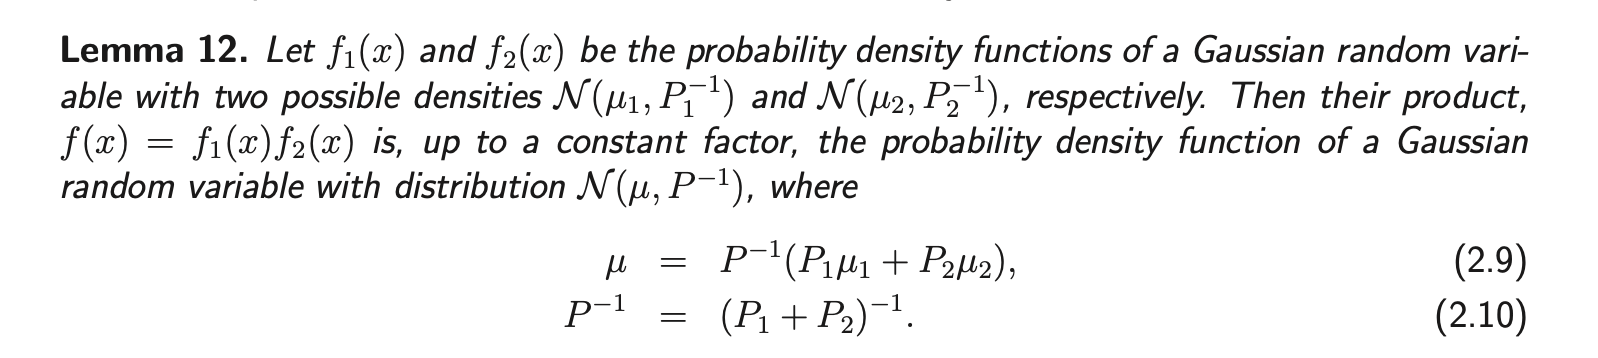
\includegraphics[width=\textwidth]{images/bickson_lemma_12}
\caption{Lemma 12 of \cite{bickson2008gaussian}}
\label{fig:lemma_twelve_bickson}
\end{figure}

\section{The Inverse Wishart Distribution} \label{sec:inverse_wishart_distribution}
 
The Inverse Wishart is a distribution on symmetric,  positive definite matrices.     The Inverse Wishart distribution,  denoted $\InverseWishart(\nu, \+\Psi)$,  has density

\begin{align}
p(\+\Sigma) \propto | \+\Sigma|^{-(\nu+d +1) /2}  \exp \bb{ -\df{1}{2} \tr ( \+\Sigma^{-1} \+\Psi) } 
\label{eqn:inverse_wishart_density}
\end{align}
where $\+\Sigma \succ 0$ and $\nu > d-1$ to have a proper prior.     The expected value of an Inverse Wishart random variable parametrized as in \eqref{eqn:inverse_wishart_density} is given by $\E[\+\Sigma] = \frac{\+\Psi}{\nu -d -1}$.   

\begin{remark}{\remarktitle{Interpreting the parameters of the Inverse Wishart}}
\label{rk:inverse_wishart_parameter_interpretation}
Note that the parameters of the Inverse Wishart can be interpreted (as per conjugacy;  see \eqref{eqn:Sigma_cc_normal_model_cond_conj_prior}) in the following way: the covariance was estimated from $\nu$ observations with a residual sum of squares (a.k.a.  sum of pairwise deviation products) $\+\Psi$. 
 
\end{remark}

Remark \ref{rk:inverse_wishart_parameter_interpretation} also provides inuition on the expected value.      For a visualization of how samples are affected by the parameters,  see \cite{hughes2012inverse}. 

\begin{remark}{\remarktitle{Peter Hoff's notation for the Inverse Wishart: A warning}}
\label{rk:peter_hoffs_notation_for_inverse_wishart}
Note that some authors (e.g.  \cite{hoff2009first},  pp.257) use the notation $\InverseWishart(\nu,  \+M)$ to refer to the density under reparametrization
\begin{align}
p(\+\Sigma) \propto | \+\Sigma|^{-(\nu+d +1) /2}  \exp \bb{ -\df{1}{2} \tr ( \+\Sigma^{-1} \+M^{-1}) } 
\label{eqn:inverse_wishart_density_hoff}
\end{align}
and therefore appropriately altered normalization constant.  The expected value of an Inverse Wishart random variable parametrized as in   \eqref{eqn:inverse_wishart_density_hoff},  is given by $\E[\+\Sigma] = \frac{\+M^{-1}}{\nu -d -1}$.     

However,  Hoff later introduces the reparametrization $\+S := \+M^{-1}$,  and so writes $\InverseWishart(\nu, \+S^{-1})$ to mean 
\begin{align}
p(\+\Sigma) \propto | \+\Sigma|^{-(\nu+d +1) /2}  \exp \bb{ -\df{1}{2} \tr ( \+\Sigma^{-1} \+S) } 
\label{eqn:inverse_wishart_density_hoffs_alternate}
\end{align}
which is \eqref{eqn:inverse_wishart_density}, and which we would write as $\InverseWishart(\nu, \+S)$.
 
\end{remark}

\begin{remark}{\remarktitle{Comparing parametrizations}}
Regarding Remark \ref{rk:peter_hoffs_notation_for_inverse_wishart},  prefer our notation because 
\begin{itemize}
\item It is the natural parameterization (see Example \ref{ex:inverse_wishart_as_ef}).
\item It lets $\+\Psi$ be interpreted directly as a prior residual sum of squares (see Remark \ref{rk:inverse_wishart_parameter_interpretation}). 
\item It matches the parametrization used throughout Wikipedia,  e.g. in its conjugacy tables.
\end{itemize}
 
\end{remark}



\subsection{Relation to other distributions}
The Wishart distribution has the same support as the Inverse Wishart;  however,  the Wishart does not give a conditionally conjugate prior on the covariance of a normal distribution.    The Inverse Wishart density can be derived from the Wishart via the multivariate change of variables  \cite{wolpert2011change}. \footnote{It is claimed in Wikipedia that if $\+X \sim \Wishart(\nu,  \+\Psi)$  then $\+X^{-1} \sim \InverseWishart(\nu,  \+\Psi^{-1})$.   I almost was able to show this using the multivariate change of variables  \cite{wolpert2011change} along with (15.15) of \cite{dwyer1967some},  but I  was off by a negative when attempting to combine the two terms with $|\+X^{-1}|$ raised to an exponent.}\redfootnote{TO DO: Provide derivation.}

In particular,  we have the relation $\+\Sigma \sim \InverseWishart(\nu, \+\Psi) \implies \+\Sigma^{-1} \sim \Wishart(\nu,  \+\Psi^{-1})$.    Thus,  if covariance matrix $\+\Sigma$ has this Inverse Wishart distribution,  then we obtain the expected value of the precision matrix as $\E[\+\Sigma^{-1}] = \nu \+\Psi^{-1}$.

The inverse Wishart can be seen as a generalization of the inverse gamma distribution to multiple dimensions.\redfootnote{TODO: fill in.   Make explicit how it is a generalization.}


\subsection{Entropy and relative entropy}

Let $\+\Sigma$ have an Inverse Wishart distribution (parametrized to have density \eqref{eqn:inverse_wishart_density}).  Then its entropy is given by \cite{gupta2010parametric}:

\begin{align*}
\H(\+\Sigma) = \ln \Gamma_d \bigg(\frac{\nu}{2} \bigg) + \frac{\nu d}{2}
+ \frac{d+1}{2} \ln \bigg| \frac{\+\Psi}{2} \bigg| - \frac{\nu + d+ 1}{2} \sum_{i=1}^d \psi \bigg( \frac{\nu - d + i}{2} \bigg)
\end{align*}
where $\psi$ denotes the digamma function,  $\psi(x) = \frac{d}{dx} \Gamma(x)$.\redfootnote{It is unfortunate that in our notation,  $\+\Psi$ and $\psi$ mean completely different things;  fix this.}

The relative entropy between two Inverse Wishart distributions $p_1, p_2$ with parameters $\nu_1,  \+\Psi_1$ and $\nu_2,  \+\Psi_2$ is given by \cite{gupta2010parametric}:

\begin{align*}
\KL{p_1}{p_2} &= \ln \bigg( \df{\Gamma_d ( \frac{\nu_2}{2})}{\Gamma_d (\frac{\nu_1}{2})} \bigg) + \df{\nu_1}{2} \tr(\+\Psi_1^{-1} \+\Psi_2) - \df{\nu_1 d}{2} - \df{\nu_2}{2} \ln \bigg| \+\Psi_1^{-1} \+\Psi_2 \bigg| - \df{\nu_2 - \nu_1}{2}\sum_{i=1}^d \psi \bigg( \frac{\nu_1 - d + i}{2}  \bigg)
\end{align*}

\subsection{Sampling}

A sample $\+\Sigma$ from the $\InverseWishart(\nu, \+\Psi)$ distribution (using the natural parametrization of \eqref{eqn:inverse_wishart_density}) can be obtained by the following scheme\redfootnote{TODO: Provide derivation of this scheme.  See perhaps \url{https://www.math.wustl.edu/~sawyer/hmhandouts/Wishart.pdf}.} \cite{hoff2009first}:

\begin{enumerate}
\item Sample $\+z_1, ..., \+z_{\nu} \iid \N (\+0,  \+\Psi^{-1})$
\item Calculate $\+Z^\top \+Z = \sum_{i=1}^\nu \+z_i \+z_i^\top$.
\item Set $\+\Sigma = ( \+Z^\top \+Z )^{-1}$.
\end{enumerate}
The intuition is that the Inverse Wishart models covariance matrices as an inverse sum of squares (again, see Remark \ref{rk:inverse_wishart_parameter_interpretation}).  

\subsection{Evaluation as a model for covariance matrices}

The  Inverse Wishart is a popular choice for modeling covariance matrices (e.g.  see \cite{hoff2009first}),  due to at least the fact that is a  conditionally conjugate prior on the covariance of a normal distribution.   (See Section \ref{sec:normal_data_with_non_conjugate_prior}.)   It seems to me that a weakly informative prior could be constructed by setting  $\nu = d+2$ (the smallest integer for which $\nu$ is in the parameter space) and $\+\Psi = (\nu -d - 1) \+I = \+I$.   This would presumably be reasonable at least if one expected unit variances and wanted to make a prior assumption of independence across dimensions.

Some problems with the Inverse Wishart as a model for covariance matrices is summarized in  \cite{alvarez2014bayesian}.    We highlight that:
\begin{enumerate}
\item  When $\nu  > 1$,   the implied scaled inv-$\chi^2$ distribution on the individual variances has extremely low density in the region near zero.   
\item The prior imposes a dependency between the correlations and the variances. In particular,  larger variances are associated with absolute values of the correlations near 1 while small variances
are associated with correlations near zero.    
\end{enumerate}
For additional discussion on the problems with Inverse Wishart,  especially when used in hierarchical models,  and for a remedy using a half-t distribution that also has a conditionally conjugate construction,  see \cite{wojnowicz2022categorical}.


\section{General Conjugacy Formalism: Alternate Approaches}

\subsection{General Conjugacy Formalism: Alternate Approach 1\footnote{This argument follows the argument (and notation) of \cite{johnson2016composing}, Appendix B.  As of now, I find it more intuitive then the argument given in the main body.}}
\label{sec:general_conjugacy_alternate_argument}


Let $p(y \cond \theta)$ be an exponential family likelihood, and let $p(\theta)$ be its conjugate prior. 

We can write the prior as 
\begin{align*}
p(\theta ) &= \exp \biggset{\biggip{\eta_\theta^o}{\sufficientStatsFunction_\theta (\theta)} - \log Z_\theta(\eta_\theta^o)} 
%&\propto \exp \biggset{\biggip{\eta_\theta^o, \sufficientStatsFunction_\theta (\theta)}}
\end{align*}

And the likelihood for a single observation $y_i$ as 
\begin{align*}
p(y_i \cond \theta)  & \stackrel{1}{=} \exp \biggset{ \biggip{\eta_y(\theta)}{\sufficientStatsFunction_y(y_i)} - \log Z_y (\eta_y(\theta)) } \\
& \stackrel{2}{=} \exp \biggset{ \biggip{ \bigparenth{\eta_y(\theta), \; - \log Z_y (\eta_y(\theta))}}{\bigparenth{\sufficientStatsFunction_y(y_i), \; 1}}  } \\
& \stackrel{3}{=} \exp \biggset{ \biggip{\sufficientStatsFunction_\theta(\theta)}{\bigparenth{\sufficientStatsFunction_y(y_i),1}}}   
\end{align*}
where (1) is true by the exponential family assumption, (2) regroups terms to make conjugacy clearer and (3) must be true given conjugacy. 


By Bayes law, the posterior after a single observation $y_i$ is given by
\begin{align*}
p(\theta \cond y_i)  &\propto p(\theta, y_i) \\
	&=\exp \biggset{ \biggip{ \eta_\theta(y_i)}{\sufficientStatsFunction_\theta(\theta) } - \log Z_\theta(\eta_\theta^o)} 
\end{align*}
where $\eta_\theta(y_i) = \eta_\theta^o + \bigparenth{\sufficientStatsFunction_y(y_i),1}$, i.e. the posterior natural parameter is the sum of the prior natural parameter and the sufficient statistics concatenated with the number of samples. 

And so after re-normalizing
\begin{align*}
p(\theta \cond y_i)  = \exp \biggset{ \biggip{ \eta_\theta(y_i)}{\sufficientStatsFunction_\theta(\theta) } - \log Z_\theta \big(\eta_\theta(y_i)\big)}
\labelit \label{eqn:posterior_for_exponential_family_after_one_obs} 
\end{align*}
  
After seeing multiple i.i.d observations $y=(y_1,...,y_n)$ from the likelihood, the posterior is given by
\begin{align*}
p(\theta \cond y)  = \exp \biggset{ \biggip{\eta_\theta(y)}{\sufficientStatsFunction_\theta(\theta) } - \log Z_\theta \big(\eta_\theta(y)\big)} 
\labelit \label{eqn:posterior_for_exponential_family_after_many_obs} 
\end{align*}
where $\eta_\theta(y) = \eta_\theta^o + \bigparenth{ \sum_{i=1}^n \sufficientStatsFunction_y(y_i),n}$.

This motivates interpreting the prior parameter as $\eta_\theta = (\tau_0, n_0)$, where $\tau_0 \in \R^{\dim(\eta_\theta) - 1}$ is interpreted as sufficient statistics and $n_0 \in \R$ is interpreted as a the sample size of a prior psuedo-dataset. 


Note that this argument yields the same parameter updating scheme of \eqref{eqn:general_formalism_prior_to_posterior_conversion}.


\subsection{Alternate approach 2} \label{sec:ef_general_formalism_jordan}

Following \cite{jordan2010conjugate}, here we provide a general formalism for conjugate priors for exponential family data models. 

Writing the exponential family density in canonical form, we have
\[ p(x \cond \naturalParam) = \carrierDensity(x) \exp \{ \naturalParam^\top T(x) - A(\naturalParam) \} \]
where $\naturalParam$ is the canonical parameter, $T(x)$ are the sufficient statistics,  $\carrierDensity(x)$ is the carrier density, and $A(\naturalParam)$ is the log normalizer (and so is \textit{not} a degree of freedom). 

The natural parameter space is 
\[  \bigg\{\naturalParam : \ds\int \carrierDensity(x) \exp \{ \naturalParam^\top T(x) - A(\naturalParam) \} < \infty \bigg \}\]

Given a random sample, $\+x=(x_1, x_2, .., x_N)$, we obtain:
\[ p(\+x \cond \naturalParam) = \bigg( \ds\prod_{i=1}^N \carrierDensity(x_i)  \bigg) \exp \bigg\{ \naturalParam^\top  \ds\sum_{i=1}^N T(x_i) - N A(\naturalParam) \bigg\} \]
as the likelihood function.

A conjugate prior can be obtained by mimicking the likelihood
\begin{equation}
p (\naturalParam \cond \tau, n_0) = H(\tau, n_0) \exp \{ \tau^\top \naturalParam - n_0 A(\naturalParam)\}
\label{eqn:conjugate_prior_exptl_family}
\end{equation}

where now $H(\tau, n_0)$ is the normalizing factor.  (For conditions on normalizability, see \cite{jordan2010conjugate}).   Note that $\tau$ has the dimensionality of the canonical parameter $\naturalParam$ and $n_0$ is a scalar.

To verify conjugacy, we compute the posterior density
\[ p (\naturalParam \cond \+x, \tau, \naturalParam_0)  \propto \exp \bigg\{ \bigg( \tau + \ds\sum_{n=1}^N  T(x_n) \bigg)^\top \naturalParam - (n_0 + N) A(\naturalParam) \bigg\} \]
which retains the form of \eqref{eqn:conjugate_prior_exptl_family}.  For an argument that is perhaps more intuitive, see Section \ref{sec:general_conjugacy_alternate_argument} 

Thus, the prior-to-posterior conversion can be summarized with the following update rules
\begin{align*}
\tau & \to \tau + \ds\sum_{n=1}^N T(x_n) \\
n_0 & \to  n_0 + N \\
\labelit \label{eqn:general_formalism_prior_to_posterior_conversion}
\end{align*}

For conjugate Bayesian models, the predictive posterior distribution, $p(x_{\text{new}} \cond x)$ is always tractable, because it has the same form (integrating a likelihood against the parameter distribution) as does the evidence term in Bayes law.   For exponential family models, the predictive posterior takes the form of a ratio of normalizing factors

\begin{equation}
p(x_{\text{new}} \cond x) = \df{H(\tau_{\text{post}}, n_0 + N)}{H(\tau_{\text{post}} + T(x_{\text{new}}), n_0 + N + 1)}
\label{eqn:predictive_posterior_exptl_family}
\end{equation}

For a proof of this, see Sec.~\ref{sec:posterior_predictives}.

\red{TODO:  Redo some of the examples using the exponential family conjugate prior formalism.    A possibly useful resource in the giant table at \url{https://en.wikipedia.org/wiki/Exponential_family}.}

\section{Posterior Predictives} \label{sec:posterior_predictives}

\input{/Users/miw267/Repos/changepoints_notes/inputs/posterior_predictives}

\section{Bayesian networks} \label{sec:bayesian_networks}


\subsection{Overview}

\input{/Users/miw267/Repos/minis/pgms/bayesian_network}


\subsection{Markov blankets} \label{sec:markov_blankets}

\input{/Users/miw267/Repos/minis/pgms/markov_blankets_and_complete_conditionals}




\section{Bayesian multivariate linear regression: Alternate derivations}  \label{sec:more_bayesian_multivariate_linear_regression} 


Below we give two alternate proofs for the posterior of the regression weights in multivariate linear regression,  compared to what was given in Proposition \ref{prop:bayes_linear_regression_with_known_ssq}.  

We begin by restating the proposition here,  then we provide the alternate proof.

\begin{proposition} \label{prop:bayes_linear_regression_with_known_ssq}
Consider the Bayesian linear multiple regression model with known observation noise $\sigma^2$
\begin{align*}
\+\beta &\sim \N (\+\mu_0, \+\Sigma_0) \\
y_i \cond \+\beta &\indsim \N (\+x_i^\top \+\beta, \sigma^2),  \quad i=1,...,n \\
\labelit \label{eqn:bayesian_multiple_linear_regression_with_known_observation_noise_APPENDIX}
\end{align*}
where  $\+x_i$ designates the $i$-th row of the design matrix $\+X \in \R^{n \times p}$.

The posterior distribution for \eqref{eqn:bayesian_multiple_linear_regression_with_known_observation_noise} is given by 
\begin{align*}
\+\beta \cond \+y & \sim \N(\+\mu,  \+\Sigma )
\intertext{where}
\+\Sigma &= \bp{\+\Sigma_0^{-1} +  \frac{1}{\sigma^2} \+X^\top \+X }^{-1}  \\
\+\mu &= \+\Sigma \bp{   \+\Sigma_0^{-1} \+\mu_0 +  \frac{1}{\sigma^2} \+X^\top  \+y}  \\
\labelit \label{eqn:posterior_bayesian_lin_regression_with_known_obs_var_APPENDIX}
\end{align*}

\end{proposition}


\begin{proof}
By Bayes rule,
\begin{align*} 
p(\+\beta \cond \+y) &\propto   p(\+\beta)  \exp \bigg\{  \ds\sum_{i=1}^N  -\frac{1}{2 \sigma^2} \bigg( y_i -  \+x_i^\top \+\beta \bigg)^2  \bigg\} \\
\intertext{and defining $\+\Omega  \in \R^{n \times n}: \+\Omega = \text{diag} (\frac{1}{\sigma^2}, ..., \frac{1}{\sigma^2})$,  we have} 
&\stackrel{1}{\propto}  p(\+\beta)   \exp \bigg\{  -\half  (\+y - \+X \+\beta)^\top \+\Omega   (\+y - \+X \+\beta) \bigg\} \\ 
&\stackrel{2}{\propto}  p(\+\beta)   \exp \bigg\{  -\half  (\+X^+ \+y - \+\beta)^\top  \+X^\top \+\Omega \+X   (\+X^+ \+y - \+\beta) \bigg\} 
\end{align*}
where (1) writes the weighted sum of squares in matrix notation, and (2) isolates $\+\beta$,  using $\+X^{+}$,  the Moore-Penrose psuedo-inverse of $\+X$. \footnote{Specifically,  since $\+X\+X^+ = \+I$,  we use 
\begin{align*}
(\+y - \+X \+\beta)^\top \+\Omega   (\+y - \+X \+\beta) &= (\+X\+\beta - \+y)^\top \+\Omega (\+X\+\beta - \+y)\\ &= \bigg( \+X (\+\beta - \+X^+ \+y ) \bigg)^\top \+\Omega  \bigg(  \+X (\+\beta - \+X^+ \+y ) \bigg) \\
&= (\+\beta - \+X^+ \+y)^\top \+X^\top \+\Omega \+X   (\+\beta - \+X^+ \+y) 
\end{align*}
.}  

Thus,  we see that $p(\+\beta \cond  \+y)$ is proportional to the product of two multivariate Gaussians:  $p(\+\beta)$,  which has mean $\+\mu_0$ and covariance $\+\Sigma_0$,  and another Gaussian,  which has mean $\+X^+ \+y$ and covariance $(\+X^\top \+\Omega \+X)^{-1}$.   We know from the exponential family representation of the Gaussian that the resulting distribution can be obtained by summing at the scale of natural parameters -- which for the Gaussian are the precision and precision-weighted mean. \footnote{See,  for reference,  Section \ref{sec:mvn_in_message_passing}.}   Using this,  we obtain

\begin{align*}
p(\+\beta \cond \+y) & \sim \N(\+\mu,  \+\Sigma )
\intertext{where}
\+\Sigma &= \bp{\+\Sigma_0^{-1} +  \+X^\top \+\Omega \+X }^{-1}  \\
\+\mu &= \+\Sigma  \bp{   \+\Sigma_0^{-1} \+\mu_0 + \+X^\top \+\Omega \cancel{\+X} \cancel{\+X^+}  \+y }  \\
&= \+\Sigma \bp{   \+\Sigma_0^{-1} \+\mu_0 + \+X^\top \+\Omega \+y}  
\end{align*}

recalling that we defined $\+\Omega = \text{diag} (\frac{1}{\sigma^2}, ..., \frac{1}{\sigma^2})$ completes the proof. 
\end{proof}


Now we provide a third proof,  which may be of interest.   Whereas both proofs of proposition \ref{prop:bayes_linear_regression_with_known_ssq} that we have seen so far (both the proof given in Section  \ref{sec:Bayesian_linear_regression_with_normal_prior}, as well as the one given immediately above)  refer to exponential family properties,  the proof below does not,  and instead uses multivariate completing the square to do the heavy lifting. 

Note that proposition 
\ref{prop:bayes_linear_regression_with_known_ssq_and_zero_prior_mean} below, as stated,  is slightly more restrictive in that it assumes the prior mean is zero.   This additional restriction is not necessary; the proposition could be rewritten to match 
Proposition \ref{prop:bayes_linear_regression_with_known_ssq} exactly,  and the proof could be adjusted accordingly to match the additional generality.    The difference in statements is just an unnecessary presentational blemish.\redfootnote{TODO: fix up the unnecessary presentational blemish -- assuming that we don't end up sacrifing too much pedagogical clarity for the sake of generality}.
%The posterior distribution for \eqref{eqn:bayesian_multiple_linear_regression_with_known_observation_noise} is given by 


\begin{proposition} \label{prop:bayes_linear_regression_with_known_ssq_and_zero_prior_mean}
Consider the Bayesian linear multiple regression model
\begin{align*}
\+\beta &\sim \N (\+0, \+V) \\
y_i \cond \+\beta &\indsim \N (\+x_i^\top \+\beta, \sigma^2),  \quad i=1,...,n
\end{align*}

where  $\+x_i$ designates the $i$-th row of the design matrix $\+X \in \R^{n \times p}$.

The posterior distribution for this model is given by 
\begin{align*}
p(\+\beta \cond \+y) & \sim \N(\+\mu,  \+\Sigma )
\intertext{where}
\+\mu &= \df{1}{\sigma^2} \+\Sigma \+X^\top \+y \\
\+\Sigma &= \bigg( \df{1}{\sigma^2}  \+X^\top \+X + \+V^{-1}  \bigg)^{-1} \\
\end{align*}
\end{proposition} 


\begin{proof}
The posterior on $\+\beta$ given $\+y = (y_1,...,y_N)^\top$ is Gaussian,  since

\begin{align*}
\ln p(\+\beta \cond \+y) &= \ds\sum_{i=1}^n \ln p(y_i \cond \+\beta)  + \ln p(\+\beta) \\
&= -\df{1}{2 \sigma^2} \ds\sum_{i=1}^n (y_i - \+x_i^\top \+\beta)^2  - \half \+\beta^\top \+V^{-1} \+\beta + \text{constant} \\
&\stackrel{1}{=} -\df{1}{2 \sigma^2} \bigg(  \+y^\top \+y - 2 \+y^\top \+X^\top \+\beta + \+\beta^\top \+X^\top \+X \+\beta \bigg)  - \half \+\beta^\top \+V^{-1} \+\beta + \text{constant} \\
&\stackrel{2}{=} -\half (\+\beta - \+\mu)^\top \+\Sigma^{-1} (\+\beta - \+\mu) +  \text{constant} \\
\intertext{where}  \\
\+\mu &= \df{1}{\sigma^2} \+\Sigma \+X^\top \+y \\
\+\Sigma &= \bigg( \df{1}{\sigma^2}  \+X^\top \+X + \+V^{-1}  \bigg)^{-1} \\
\end{align*}

Equality (1) is obtained by noting $ \sum_{i=1}^n (y_i - \+x_i^\top \+\beta)^2  = (\+y - \+X \+\beta)^\top (\+y - \+X \+\beta)$, FOIL-ing, and observing that the cross-products are scalars.   Equality (2) is obtained by completing the square,  where $\+\beta$ plays the role of $\+x$  in \eqref{eqn:multivariate_completing_the_square},  and where in that notation we have $\+M = \frac{1}{\sigma^2} \+X^\top \+X + \+V^{-1}$ and $\+b^\top = \frac{1}{\sigma^2} \+y^\top \+X^\top$.
\end{proof}


\end{document}